\documentclass[10pt,a4paper]{article}
\usepackage[T1]{fontenc}
\usepackage[utf8]{inputenc}
\usepackage[spanish,es-noquoting]{babel}
\usepackage{lmodern}
\usepackage[margin=2.3cm]{geometry}
\usepackage{amsmath,amssymb}
\usepackage{graphicx}
\usepackage{booktabs}
\usepackage{siunitx}
\usepackage{caption}
\usepackage{xcolor}
\usepackage[colorlinks=true,linkcolor=black,citecolor=black,urlcolor=blue!60!black]{hyperref}
\usepackage{textcomp}
\usepackage{microtype}
\newcommand{\doi}[1]{DOI: \href{https://doi.org/#1}{#1}}
\usepackage{fancyhdr}

\sisetup{output-decimal-marker={,}, group-separator={\,}}
\captionsetup{font=small,labelfont=bf}
\pagestyle{fancy}\fancyhf{}
\fancyhead[L]{\footnotesize Heredia Alessandrello \textperiodcentered{} Eclipse total 2026-08-12 con el Sol a \altMax\textdegree{}}
\fancyhead[R]{\footnotesize\thepage}
\renewcommand{\headrulewidth}{0.3pt}

\newcommand{\EBCOne}{24{,}0}
\newcommand{\EBlimit}{1}
\newcommand{\EBnoEclMax}{1{,}577}
\newcommand{\ERlimit}{201{,}9}
\newcommand{\EpkOneSix}{59{,}42}
\newcommand{\EpkThreeZeroZero}{18{,}34}
\newcommand{\EpkThreeZeroZeroNoon}{33{,}7}
\newcommand{\Epkphone}{201{,}63}
\newcommand{\PglobOneSix}{8}
\newcommand{\PglobThreeZeroZero}{871}
\newcommand{\PwOneSix}{8}
\newcommand{\PwThreeZeroZero}{871}
\newcommand{\Pwphone}{5}
\newcommand{\alphaSun}{9{,}18}
\newcommand{\alphaSunMrad}{9{,}18}
\newcommand{\altCOne}{14{,}70}
\newcommand{\altMax}{4{,}75}
\newcommand{\amCOne}{3{,}89}
\newcommand{\amMax}{10{,}7}
\newcommand{\amSpread}{2{,}9}
\newcommand{\aodFiveFiveZero}{0{,}16}
\newcommand{\azMax}{285{,}7}
\newcommand{\bestDur}{100}
\newcommand{\clearance}{5{,}17}
\newcommand{\cloud}{0}
\newcommand{\concFOneNine}{3288}
\newcommand{\concFSixThree}{299}
\newcommand{\concMax}{47475}
\newcommand{\dTglobOneSixHi}{0{,}4}
\newcommand{\dTglobOneSixLo}{0{,}1}
\newcommand{\dTglobThreeZeroZeroHi}{43{,}6}
\newcommand{\dTglobThreeZeroZeroLo}{8{,}7}
\newcommand{\dTonedThreeZeroZero}{0{,}37}
\newcommand{\dTshutterAl}{62}
\newcommand{\dTssOneSix}{0{,}295}
\newcommand{\dTssThreeZeroZero}{1{,}706}
\newcommand{\dTssThreeZeroZeroNoon}{3{,}14}
\newcommand{\dTssphone}{0{,}433}
\newcommand{\dTworstThreeZeroZero}{6{,}83}
\newcommand{\deltaT}{69{,}099}
\newcommand{\deltaTdiff}{2{,}30}
\newcommand{\dniCOne}{489}
\newcommand{\dniMaxHigh}{186}
\newcommand{\dniMaxLow}{61}
\newcommand{\dniMaxNoEcl}{186}
\newcommand{\dniMaxSpread}{3{,}0}
\newcommand{\driftOneSix}{3{,}35}
\newcommand{\driftRate}{14{,}31}
\newcommand{\driftThreeZeroZero}{0{,}18}
\newcommand{\efold}{0{,}244}
\newcommand{\gammaPh}{11}
\newcommand{\gerr}{+2{,}09}
\newcommand{\gradient}{0{,}62}
\newcommand{\horizonAtTotality}{-0{,}42}
\newcommand{\horizonMax}{-0{,}38}
\newcommand{\imgDiaOneSix}{147}
\newcommand{\imgDiaThreeZeroZero}{2{,}75}
\newcommand{\lamSun}{139{,}694}
\newcommand{\ldAlpha}{0{,}508}
\newcommand{\ldPeak}{1{,}254}
\newcommand{\localCOne}{19:35:27}
\newcommand{\localCTwo}{20:29:25.6}
\newcommand{\localCThree}{20:30:35.9}
\newcommand{\localCFour}{21:21:19}
\newcommand{\localMax}{20:29:59.8}
\newcommand{\luxCOne}{44494}
\newcommand{\luxMaxNoEcl}{7404}
\newcommand{\magMax}{1{,}0324}
\newcommand{\marginA}{18}
\newcommand{\marginB}{2672}
\newcommand{\marginFast}{1{,}9}
\newcommand{\northLimit}{48}
\newcommand{\ordersMelt}{3{,}0}
\newcommand{\pPerseidOneSix}{0{,}31}
\newcommand{\pPerseidOneSixbest}{0{,}03}
\newcommand{\pPerseidMax}{0{,}67}
\newcommand{\partialDur}{105{,}9}
\newcommand{\perpLimit}{42}
\newcommand{\phoneRatio}{3{,}9}
\newcommand{\plungeMin}{5{,}2}
\newcommand{\psurf}{949{,}9}
\newcommand{\pw}{2{,}76}
\newcommand{\radiantAlt}{9{,}2}
\newcommand{\radiantDec}{57{,}4}
\newcommand{\radiantRA}{47{,}4}
\newcommand{\radiantSunSep}{80{,}0}
\newcommand{\reqFilterCOne}{4.16e-02}
\newcommand{\siteElevDEM}{616{,}1}
\newcommand{\siteLat}{41{,}212878}
\newcommand{\siteLon}{0{,}709488}
\newcommand{\stareCOne}{4{,}2}
\newcommand{\stareCOnePFive}{1{,}5}
\newcommand{\stareCOnePSeven}{0{,}8}
\newcommand{\stareCOnePThree}{4{,}2}
\newcommand{\stareNoEclMax}{63}
\newcommand{\stareNoEclMaxPFive}{23}
\newcommand{\stareNoEclMaxPSeven}{12}
\newcommand{\stareNoEclMaxPThree}{63}
\newcommand{\sunsetDrop}{62{,}1}
\newcommand{\tauDiffThreeZeroZero}{21}
\newcommand{\tauNinetyFiveThreeZeroZero}{0{,}67}
\newcommand{\tauSpotOneSix}{0{,}03}
\newcommand{\tauSpotThreeZeroZero}{11}
\newcommand{\thermExcessCOne}{30}
\newcommand{\thermRatioCOne}{1{,}30}
\newcommand{\thermRatioMax}{0{,}34}
\newcommand{\thermRatioPeak}{1{,}34}
\newcommand{\threshA}{323}
\newcommand{\totalityDur}{70{,}3}
\newcommand{\totalityDurBess}{59{,}2}
\newcommand{\totalityDurKTwo}{70{,}3}
\newcommand{\unlimitedFrom}{-11{,}6}
\newcommand{\unlimitedFromPSeven}{-5{,}3}
\newcommand{\unlimitedFromPThree}{-11{,}6}


\newcommand{\repourl}{https://github.com/RHA-UPC/eclipse-radiometric-simulation}

\hypersetup{
  pdftitle={Riesgo radiometrico de un eclipse total con el Sol a baja altura:
            sensores fotograficos, ojo humano y probabilidad de captar una Perseida},
  pdfauthor={Ricardo Heredia Alessandrello},
  pdfsubject={Eclipse solar total del 12 de agosto de 2026: radiometria, seguridad de sensores y limites de exposicion ocular},
  pdfkeywords={eclipse solar total; radiometria; ICNIRP; seguridad retiniana; sensor CMOS; masa de aire; Perseidas},
}

\title{\bfseries Riesgo radiométrico de un eclipse total con el Sol a \altMax\textdegree{} de altura:\\
sensores fotográficos, ojo humano y probabilidad de captar una Perseida\\[2mm]
\large Emplazamiento: observatorio republicano de la Batalla del Ebro, \siteLat\textdegree{} N, \siteLon\textdegree{} E, \siteElevDEM\,m}
\author{%
  \large Ricardo Heredia Alessandrello\\[1mm]
  \normalsize\itshape Observación de campo, Priorat, Tarragona, España
}
\date{\normalsize Observación: 12 de agosto de 2026\\[1mm]
      \footnotesize Preprint. No sometido a revisión por pares.}

\begin{document}
\maketitle

\begin{abstract}
\noindent
El eclipse total de Sol del 12 de agosto de 2026 es totalmente atípico para la
península ibérica: la totalidad ocurre con el Sol a menos de cinco grados sobre
el horizonte, media hora antes del ocaso. Ese detalle geométrico cambia por
completo el balance de riesgos respecto a un eclipse en altura, y lo cambia en
direcciones opuestas según de qué riesgo se hable. Este trabajo cuantifica tres
de ellos para un emplazamiento concreto, a partir de efemérides JPL DE440s, un
modelo digital del terreno Copernicus GLO-30, el estado atmosférico real
pronosticado para la tarde del evento y los límites de exposición ICNIRP 2013.
Los resultados principales son: el emplazamiento está dentro de la franja de
totalidad, a \perpLimit\,km del límite norte, con \totalityDur\,s de totalidad y
el Sol a \altMax\textdegree{}, y su horizonte topográfico real hacia el poniente
está deprimido, dejando \clearance\textdegree{} de margen libre. La irradiancia normal directa cae de
\dniCOne~\si{\watt\per\square\meter} en el primer contacto a
\dniMaxNoEcl~\si{\watt\per\square\meter} en el instante de la totalidad por el
simple hecho del atardecer, es decir, la atmósfera ya se ha comido el
\sunsetDrop\,\% de la señal antes de que la Luna aporte nada. Para los sensores,
la irradiancia en el plano focal depende solo del número f y no de la focal:
un móvil a f/1{,}9 concentra \concFOneNine{} soles y la réflex a f/6{,}3 solo
\concFSixThree. Aun así, el calentamiento local del silicio satura en
milisegundos y, en la idealización más desfavorable, no supera
\dTworstThreeZeroZero\,K en la peor configuración del teleobjetivo. Contrastado
con el único umbral de daño en onda continua publicado para un sensor de silicio
junto con su tamaño de mancha, y reescalado a la imagen solar mediante la
invariancia de $qa$, el margen en el peor instante de la tarde es de un factor
\marginA{} bajo la hipótesis conservadora. Un teleobjetivo de 300\,mm a f/2,8
apuntado al Sol de mediodía, en cambio, se queda en \marginFast{}: la advertencia
general está justificada, y este caso concreto no lo estaba. El análisis cubre el
sensor y no la cortinilla del obturador ni la pantalla de enfoque, que el mismo
modelo sitúa muy por encima en temperatura por ser delgadas y carecer de
sumidero, y para las que no se ha localizado literatura revisada por pares. Para el ojo, en cambio, la conclusión es la contraria y más
incómoda: el Sol sin eclipsar a \altMax\textdegree{} todavía supera los dos
límites retinianos de ICNIRP, el térmico por un \thermExcessCOne\,\% en el primer
contacto y el fotoquímico de luz azul, y permite \stareNoEclMaxPThree\,s de fijación con
pupila nominal de 3\,mm y solo \stareNoEclMaxPSeven\,s si la pupila se ha
dilatado, antes de rebasar la dosis admisible. Finalmente, la probabilidad de que una
Perseida entre en el encuadre durante la totalidad no llega al
\pPerseidMax\,\% en ninguna de las configuraciones exploradas.
\end{abstract}

\vspace{1mm}
\noindent\small\textbf{Palabras clave:} eclipse solar total; radiometría solar;
masa de aire; oscurecimiento de limbo; irradiancia en el plano focal; daño en
sensores CMOS; límites de exposición ICNIRP; riesgo retiniano; Perseidas.
\normalsize

\section{Introducción}

La cultura popular sobre eclipses solares se construyó alrededor de eclipses
observados con el Sol alto. De ahí vienen las dos advertencias que todo el mundo
ha oído: no se mira sin filtro y no se fotografía sin filtro. Ambas son ciertas
en el caso general. Lo que casi nunca se discute es qué queda de ellas cuando la
totalidad ocurre a cuatro o cinco grados sobre el horizonte, con el Sol
atravesando once veces más atmósfera que en el cenit y treinta minutos antes de
ponerse. Esa es exactamente la situación del 12 de agosto de 2026 en Cataluña, y
es la situación que este trabajo analiza.

La pregunta tiene dos mitades que conviene no mezclar. La primera es
instrumental: si se apunta una cámara al Sol parcialmente eclipsado a esa hora,
¿se daña el sensor, y en cuánto tiempo? La segunda es fisiológica: si se mira
sin filtro, ¿qué ocurre? La intuición sugiere que ambas respuestas mejoran
juntas al bajar el Sol, porque la irradiancia total baja. Los cálculos que
siguen muestran que no es así. El riesgo instrumental, que es esencialmente
térmico y por tanto proporcional a la potencia, se desploma. El riesgo ocular
dominante no es térmico sino fotoquímico, obedece a una dosis acumulada y no a
una potencia instantánea, y además va acompañado de la desaparición del reflejo
de aversión que normalmente impide mirar al Sol. La combinación es traicionera.

A esto se añade una circunstancia afortunada: el 12 de agosto de 2026 es Luna
nueva por construcción, pues un eclipse solar solo ocurre en Luna nueva, y
coincide con el máximo de las Perseidas. La idea de capturar una estrella fugaz
sobre la corona solar es atractiva y merece que se le ponga un número, aunque
ese número resulte desalentador.

Todo el análisis está referido a un punto concreto: un observatorio republicano
de la Batalla del Ebro en las cercanías de La Figuera, comarca del Priorat,
provincia de Tarragona, en \siteLat\textdegree{}\,N, \siteLon\textdegree{}\,E.
El modelo digital del terreno Copernicus GLO-30 sitúa ese punto a
\siteElevDEM\,m sobre el geoide EGM2008.

\section{Métodos}

\subsection{Geometría del eclipse}

Las circunstancias locales se calculan directamente a partir de las efemérides
planetarias y lunares JPL DE440s, sin recurrir a elementos besselianos ni a
tablas publicadas. Se obtienen las posiciones aparentes topocéntricas del Sol y
de la Luna, corregidas de tiempo-luz, aberración y deflexión, y se resuelve por
búsqueda de raíces el instante en que la separación angular aparente iguala la
suma de los radios aparentes, que da los contactos exteriores, o su diferencia,
que da los interiores. La escala de tiempo emplea los parámetros de orientación
terrestre IERS observados, de los que resulta $\Delta T = \deltaT$\,s para la
fecha. Este valor merece un comentario, porque la predicción con la que se
generaron las efemérides de eclipses de la NASA para este siglo suponía
$\Delta T = 71{,}4$\,s. La diferencia de \deltaTdiff\,s no es un detalle académico: en
términos de rotación terrestre equivale a desplazar al observador unos
0,8\,km hacia el este respecto a la sombra.

El radio lunar adoptado es una convención, no una medida, y afecta directamente
a la duración de la totalidad. Los elementos besselianos que la NASA publica
para este eclipse declaran \emph{dos} constantes y no son intercambiables:
$k_1 = 0{,}272488$ para los contactos penumbrales, C1 y C4, y
$k_2 = 0{,}272281$ para los umbrales, C2 y C3 \cite{espenak2006}. Este trabajo
aplica cada una donde corresponde. Una versión anterior usaba una sola constante
$k = 0{,}2725076$ para ambos, con lo que inflaba la totalidad en 3,8\,s.

\subsection{Horizonte topográfico}

A \altMax\textdegree{} de altura, preguntarse si el Sol está por encima del
horizonte astronómico es insuficiente: lo que importa es si está por encima de
la línea de cresta real. El perfil del horizonte se construye muestreando el
modelo digital de superficie Copernicus GLO-30 a lo largo de radiales cada
0,25\textdegree{} de acimut entre 265\textdegree{} y 300\textdegree{}, hasta
100\,km de distancia, con paso de 30\,m cerca del observador y 250\,m lejos. La
altura aparente de cada punto de terreno incorpora la curvatura terrestre y la
refracción atmosférica mediante un radio terrestre efectivo
$R_{\mathrm{ef}} = R/(1-k_r)$, y se reporta la sensibilidad para
$k_r \in [0{,}07;\,0{,}20]$.

\subsection{Estado atmosférico e irradiancia}

El estado atmosférico no se supone: se toma del análisis operativo para el punto
y el día. El espesor óptico de aerosoles a 550\,nm procede del servicio
Copernicus CAMS y vale \aodFiveFiveZero; el vapor de agua precipitable, la presión en
superficie y la nubosidad proceden del modelo IFS del ECMWF y valen
\pw\,cm, \psurf\,hPa y \cloud\,\% respectivamente. La nubosidad prevista es nula
en los tres niveles.

La masa de aire relativa emplea la fórmula de Kasten y Young
\cite{kastenyoung1989}, evaluada sobre la altura solar refractada. A
\altMax\textdegree{} la masa de aire vale \amMax, un régimen en el que los
modelos empíricos de banda ancha de cielo claro operan muy fuera de su rango de
ajuste. Por eso el cálculo primario es espectral: se emplea SPECTRL2
\cite{birdriordan1984}, que resuelve la extinción longitud de onda a longitud de
onda mediante ley de Beer-Lambert, la ruta defendible a masa de aire alta aunque
emplee una única masa de aire relativa también para aerosoles y vapor de agua,
lo que sesga la irradiancia al alza y por tanto del lado conservador, y que además es imprescindible para las ponderaciones biológicas. La
implementación se valida contra el espectro de referencia ASTM G173: reproduce
su integral directa con un error de \gerr\,\%.

La atenuación producida por la Luna no es la fracción de área cubierta. El
disco solar está oscurecido hacia el limbo, y la Luna lo tapa precisamente
empezando por el limbo, de modo que el déficit de flujo va por detrás del
déficit geométrico durante las fases parciales tempranas y lo adelanta cuando
la Luna alcanza el centro. Se emplea la ley de potencia de Hestroffer y Magnan
\cite{hestroffer1998}, $I(\mu)/I(1) = \mu^\alpha$ con
$\alpha(\lambda)$ dado por su ecuación 5, que a 550\,nm vale \ldAlpha. La
integral de solapamiento se reduce a una cuadratura radial unidimensional
exacta. Como $\alpha$ depende de la longitud de onda, la transmisión del
eclipse es cromática y se calcula para cada banda espectral.

\subsection{Irradiancia en el plano focal}

Para una fuente extendida, la irradiancia en el plano focal de un objetivo es
\begin{equation}
E_{\mathrm{img}} \;=\; \pi\,L\,\tau\,\sin^{2}\theta' \;=\; \frac{\pi L \tau}{4N^{2}},
\label{eq:focal}
\end{equation}
donde $L$ es la radiancia de la fuente, $\tau$ la transmitancia del objetivo y
$N$ el número f de trabajo. La irradiancia depende del número f y no depende de
la focal. Un teleobjetivo de 300\,mm a f/6,3 deposita exactamente los mismos
vatios por centímetro cuadrado que un gran angular de 16\,mm a f/6,3; lo que
cambia con la focal es el tamaño de la imagen solar, y por tanto la potencia
total y la facilidad con que el calor escapa lateralmente del punto iluminado.
La radiancia se obtiene de la irradiancia normal directa mediante el ángulo
sólido \emph{proyectado} del disco, $\Omega = \pi\sin^{2}\alpha_r$, que es la
relación exacta para un disco visto normalmente. El centro del disco es más
brillante que la media en el factor $(\alpha+2)/2 = \ldPeak$ para la ley de
oscurecimiento de limbo adoptada, y es ese valor de pico el que se usa en todos
los cálculos térmicos.

Como cota de seguridad se emplea $\tau = 1$, la elección conservadora, ya que un
objetivo perfectamente transmisor entrega al sensor la máxima energía posible.
No existe medida publicada de transmitancia o número T para el Tamron
16--300\,mm, de modo que cualquier valor concreto sería inventado; el uso de
$\tau=1$ evita el problema y garantiza que las conclusiones de seguridad no
dependen de él.

\subsection{Modelo térmico del sensor}

Actúan dos vías de calor en escalas de tiempo muy distintas y ambas hacen falta.
La primera es la constricción local. La imagen solar es un disco de radio $a$
que inyecta un flujo $q$ en el silicio, y la solución clásica de Carslaw y
Jaeger \cite{carslawjaeger} para un disco uniformemente calentado sobre un
sólido semiinfinito da la temperatura en el centro
\begin{equation}
\Delta T_c(t) \;=\; \frac{2q}{k}\sqrt{\kappa t}
\left[\frac{1}{\sqrt{\pi}} - \operatorname{ierfc}\!\left(\frac{a}{2\sqrt{\kappa t}}\right)\right],
\label{eq:cj}
\end{equation}
que crece como $\sqrt{t}$ al principio y \emph{satura} en
$\Delta T_c(\infty) = qa/k$. El tiempo característico es
$a^{2}/\kappa = \tauDiffThreeZeroZero$\,ms para la imagen solar de
\imgDiaThreeZeroZero\,mm que produce el teleobjetivo a 300\,mm. La aproximación
a la asíntota no es exponencial sino con cola $1-a/(2\sqrt{\pi\kappa t})$: el
63\,\% se alcanza a los \tauSpotThreeZeroZero\,ms y el 95\,\% a los
\tauNinetyFiveThreeZeroZero\,s. En cualquier caso, pasado alrededor de un
segundo la temperatura local está en su asíntota y deja de importar cuánto tiempo
se mantenga el obturador abierto.

La segunda vía es el calentamiento global del dado y del encapsulado por la
potencia total absorbida, que sí crece con el tiempo de exposición y cuya
constante de tiempo es de segundos a minutos. Como no se dispone de un valor
publicado de la resistencia térmica del conjunto sensor-cuerpo para esta cámara
concreta, ese término se reporta de forma paramétrica.

La dependencia con el tamaño de la mancha en la ecuación~\eqref{eq:cj} explica
por qué es incorrecto comparar directamente un umbral de daño publicado en
\si{\watt\per\square\centi\meter} con la irradiancia de una imagen solar: los
umbrales de laboratorio se miden con manchas láser de decenas de micrómetros, y
para un flujo dado $qa/k$ es cien veces menor ahí que en una imagen solar
milimétrica. La comparación correcta es entre temperaturas, no entre
irradiancias.

La figura~\ref{fig:plane} convierte esa observación en un instrumento. Como
$\Delta T = qa/k$, en el plano (radio de mancha, irradiancia absorbida) las
líneas de incremento constante son rectas de pendiente $-1$ en ejes
logarítmicos. Cualquier umbral publicado, medido con la mancha que sea, entra en
ese plano como un punto, y su recta isoterma dice a qué irradiancia equivale
para cualquier otro tamaño de mancha. Las configuraciones ópticas de este
trabajo entran también como puntos, de modo que la distancia vertical entre unos
y otros \emph{es} el margen. La franja sombreada corresponde a incrementos de
150 a 250\,K, el orden en que degradan los materiales no silíceos del apilado;
se dibuja porque es la magnitud relevante, y se rotula como no citada porque
este trabajo no localizó una fuente para ella.

Conviene ver en esa figura por qué la comparación ingenua falla. Las manchas
láser de laboratorio ocupan la banda gris de la izquierda, unas decenas de
micrómetros; la imagen solar del teleobjetivo está casi tres décadas a la
derecha. Un umbral expresado en vatios por centímetro cuadrado y trasladado sin
corregir de una a otra se equivoca en ese mismo factor, y se equivoca en la
dirección insegura.

\begin{figure}[htbp]\centering
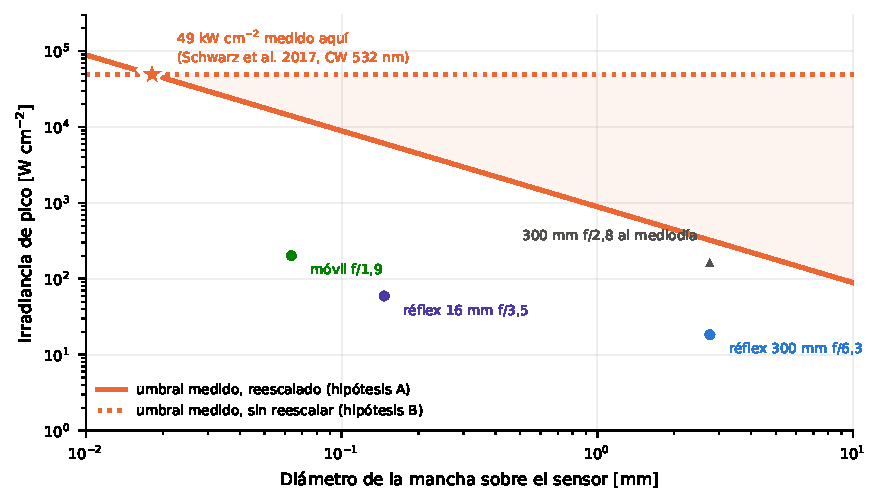
\includegraphics[width=0.9\textwidth]{../figs/fig11_threshold_plane.pdf}
\caption{Plano de comparación entre umbrales. Las rectas son incrementos de
temperatura constantes, $\Delta T = qa/k$. Los puntos son las configuraciones
ópticas analizadas, en las condiciones del primer contacto. Un umbral de daño
publicado se situaría como un punto más y su recta isoterma permitiría leer
directamente el margen; ninguno se ha localizado, y esa ausencia es la principal
limitación declarada de este trabajo.}
\label{fig:plane}
\end{figure}

Las propiedades del silicio empleadas son
$k = 148$~\si{\watt\per\meter\per\kelvin} \cite{glassbrenner1964},
$\rho = 2329$~\si{\kilo\gram\per\cubic\meter} y
$c_p = 700$~\si{\joule\per\kilo\gram\per\kelvin}, de donde
$\kappa = 9{,}08\times10^{-5}$~\si{\square\meter\per\second}.

\subsection{Riesgo ocular}

Se aplican las directrices ICNIRP 2013 \cite{icnirp2013}. Actúan dos límites
independientes. El límite térmico retiniano se rige por la radiancia ponderada
con la función $R(\lambda)$ y, para exposiciones de 0,25\,s o más, vale
$L_R^{EL} = 2{,}8\times10^{4}\,\alpha^{-1}$~\si{\watt\per\square\meter\per\steradian}.
El límite fotoquímico de luz azul se rige por la irradiancia ponderada con
$B(\lambda)$ y es una \emph{dosis}: $H_B \le 100$~\si{\joule\per\square\meter}
para exposiciones entre 0,25 y 100\,s, y $E_B \le 1$~\si{\watt\per\square\meter}
a partir de 100\,s.

Como el diámetro angular del Sol, \alphaSunMrad\,mrad, es menor que el ángulo de
aceptación $\gamma_{ph} = \gammaPh$\,mrad que ICNIRP prescribe para exposiciones
por debajo de 100\,s, el límite \emph{fotoquímico} se reduce a su forma en
irradiancia corneal. El \emph{térmico} no se reduce de la misma manera, y aquí
conviene ser explícito sobre dos errores que una revisión independiente encontró
en la versión anterior de este trabajo.

El primero es que $\alpha$ en $L_R^{EL} = 2{,}8\times10^{4}\,\alpha^{-1}$ es el
diámetro angular \emph{de la fuente}; $\gamma_{ph}$ pertenece al límite
fotoquímico y no tiene papel aquí. Evaluar el límite en 11\,mrad en lugar de en
\alphaSunMrad\,mrad sobrestimaba la radiancia permitida en un factor 1,20. Con
el diámetro correcto, la irradiancia corneal equivalente es
\ERlimit~\si{\watt\per\square\meter} y no los 241,9 que se publicaron antes.

El segundo es más de fondo. La versión anterior escalaba la \emph{radiancia}
ponderada por la transmisión del eclipse, con lo que el peligro térmico tabulado
se desvanecía según la obscuración se acercaba a la unidad. Eso contradice la
física que el propio trabajo enuncia unas páginas más adelante: la Luna quita
área, no radiancia. Un Sol cubierto al 99\,\% sigue proyectando un creciente
cuya irradiancia retiniana es la de la fotosfera completa, y por eso ICNIRP
escribe el límite térmico retiniano como un límite de \emph{radiancia}. El
tratamiento correcto mantiene la radiancia fotosférica fija, atenuada solo por la
atmósfera, y deja que responda $\alpha$, tomado como la media aritmética de las
dimensiones mayor y menor del creciente visible, cada una acotada al intervalo
$[1{,}5;\,100]$\,mrad que prescribe la guía.

\subsection{Perseidas}

Los parámetros de la lluvia proceden del calendario 2026 de la International
Meteor Organization \cite{imo2026}: máximo el 13 de agosto entre las 02 y las
04\,UT, ZHR de 100, índice de población $r = 2{,}2$, radiante en
$\alpha = 48$\textdegree, $\delta = +58$\textdegree{} y velocidad geocéntrica de
59~\si{\kilo\meter\per\second}. La posición del radiante para el 12 de agosto,
\radiantRA\textdegree{} y \radiantDec\textdegree, se interpola de la tabla 6 del
mismo documento. La longitud solar en el instante de la totalidad,
\lamSun\textdegree{} referida al equinoccio J2000,0, se calcula de la efeméride;
el marco J2000 se verifica reproduciendo el propio ancla del calendario, que
sitúa el máximo en 140,0--140,1\textdegree{} el 13 de agosto entre las 02 y las
04\,UT.

La tasa esperada dentro del encuadre se obtiene invirtiendo la definición de ZHR
y repartiendo los meteoros sobre el hemisferio visible, y de ahí la probabilidad
de al menos un suceso por estadística de Poisson. El supuesto de reparto
uniforme sobre el cielo se declara explícitamente porque es falso en detalle:
la densidad superficial aparente de una lluvia de trayectorias paralelas depende
de la distancia angular al radiante. No se aplica ninguna corrección por ese
efecto porque no se localizó una formulación citable, y se prefiere reportar el
número sin corregir a introducir un factor sin fuente.

\section{Resultados}

\subsection{Circunstancias locales y visibilidad real}

La tabla~\ref{tab:circ} recoge las circunstancias locales. La totalidad comienza
a las \localCTwo CEST y termina a las \localCThree, con el máximo a las
\localMax. El Sol está entonces a \altMax\textdegree{} sobre el horizontal, en
acimut \azMax\textdegree, y la magnitud del eclipse alcanza \magMax. El cuarto
contacto ocurre ya por debajo del horizonte: el Sol se pone todavía
parcialmente eclipsado.

\begin{table}[htbp]\centering\small
\caption{Circunstancias locales del eclipse en \siteLat\textdegree{}\,N, \siteLon\textdegree{}\,E, \siteElevDEM\,m, calculadas de JPL DE440s con $\Delta T = \deltaT$\,s y $k = 0{,}2725076$. La altura solar incluye refracción.}
\label{tab:circ}
\begin{tabular}{lccS[table-format=-2.2]S[table-format=3.1]S[table-format=1.4]S[table-format=1.4]}
\toprule
Evento & UTC & CEST & {Altura (\textdegree)} & {Acimut (\textdegree)} & {Magnitud} & {Obscuración} \\
\midrule
Primer contacto (C1) & 17:35:27.6 & 19:35:27 & 14.70 & 277.0 & 0.0000 & 0.0000 \\
Segundo contacto (C2) & 18:29:25.6 & 20:29:25 & 4.85 & 285.6 & 1.0324 & 1.0000 \\
Máximo del eclipse & 18:29:59.9 & 20:29:59 & 4.75 & 285.7 & 1.0324 & 1.0000 \\
Tercer contacto (C3) & 18:30:35.9 & 20:30:35 & 4.64 & 285.8 & 1.0000 & 1.0000 \\
Cuarto contacto (C4) & 19:21:19.2 & 21:21:19 & -4.48 & 294.1 & 0.0000 & 0.0000 \\
\bottomrule
\end{tabular}
\end{table}


La duración de la totalidad admite una comprobación cruzada exigente, y conviene
contar cómo salió porque el resultado inicial fue erróneo. El cálculo DE440s con
la convención umbral da \totalityDur\,s. Una reimplementación independiente a
partir de los elementos besselianos publicados por la NASA daba en cambio
59,2\,s, y una versión anterior de este trabajo atribuyó esa diferencia de
quince segundos a la sensibilidad extrema de una geometría rasante. Era falso.
La discrepancia era un error de una línea en la reimplementación: el ángulo
horario $\mu$ que Espenak tabula es un ángulo horario \emph{de efemérides},
referido a TDT, y convertirlo en el ángulo horario \emph{universal} del
observador exige restarle $1{,}002738\,\Delta T\times 15^{\circ}/3600$, que aquí valen
0,2983\textdegree{} de longitud, es decir 25\,km sobre el terreno. Sin ese
término la franja entera quedaba desplazada al oeste.

Corregido, el contraste es concluyente: la reimplementación reproduce las cuatro
duraciones centrales que la NASA publica para este eclipse con una desviación
máxima de 0,04\,s, y en el emplazamiento da 68,9\,s frente a los
\totalityDur\,s del cálculo DE440s. La horquilla real entre las dos soluciones
es de 1,4\,s, no de quince, y la sensibilidad extrema que dos párrafos de la
versión anterior explicaban físicamente no existía. La lección metodológica es
que la rutina de validación tenía criterio de aprobado para tres de sus cuatro
comprobaciones y ninguno para ésta, que es precisamente donde se escondía el
fallo; ahora lo tiene.

El emplazamiento está a \perpLimit\,km del límite norte de la franja medidos
perpendicularmente, y la duración crece \gradient\,s por cada kilómetro que se
avance hacia el sur (figura~\ref{fig:path}).

La visibilidad del fenómeno está asegurada desde el punto de vista topográfico.
El perfil del horizonte construido con el modelo digital de superficie
(figura~\ref{fig:horizon}) está \emph{deprimido} en todo el sector de interés:
en el acimut de la totalidad la línea de cresta real se sitúa a
\horizonAtTotality\textdegree, de modo que el Sol pasa \clearance\textdegree{}
por encima de ella. El emplazamiento domina el valle hacia el oeste-noroeste,
que es exactamente lo que se necesita.

\begin{figure}[htbp]\centering
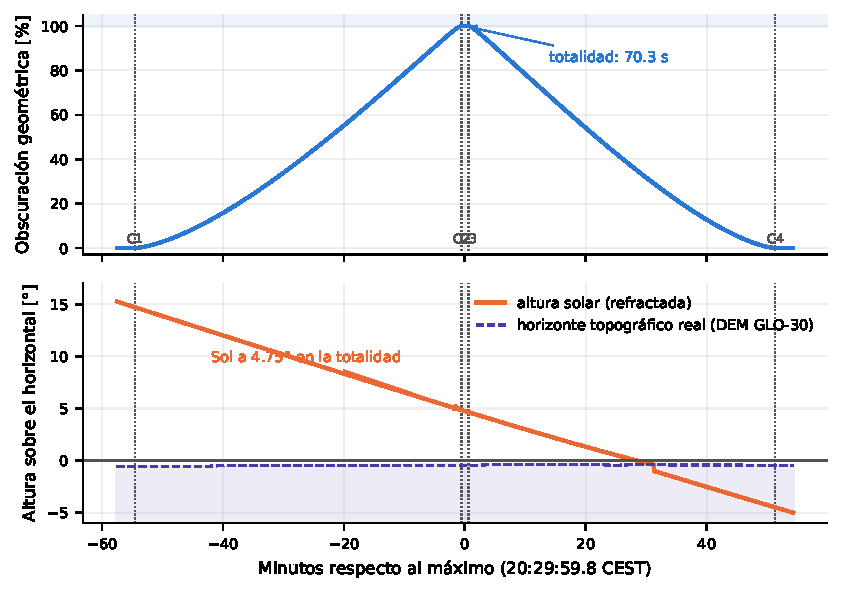
\includegraphics[width=\textwidth]{../figs/fig1_geometry.pdf}
\caption{Arriba, obscuración geométrica del disco solar. Abajo, altura del Sol
comparada con la línea de cresta real extraída del modelo digital de superficie
Copernicus GLO-30 en el acimut correspondiente a cada instante. La zona
sombreada es terreno.}
\label{fig:geom}
\end{figure}

\begin{figure}[htbp]\centering
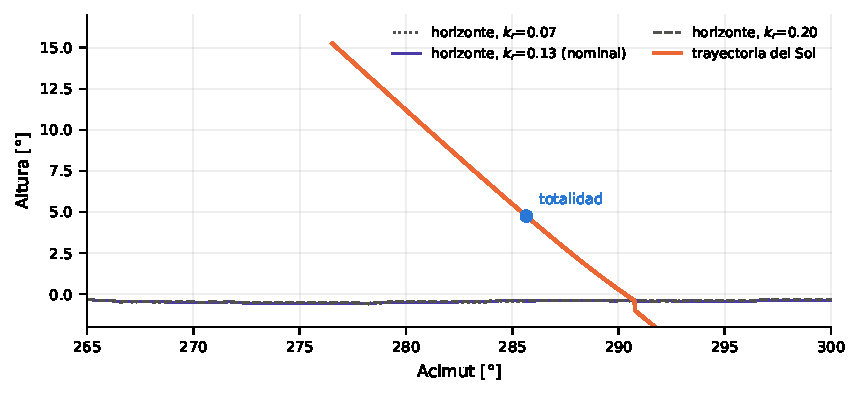
\includegraphics[width=0.86\textwidth]{../figs/fig7_horizon.pdf}
\caption{Perfil del horizonte topográfico frente a la trayectoria aparente del
Sol. Las tres curvas del horizonte corresponden a coeficientes de refracción
terrestre de 0,07, 0,13 y 0,20; la conclusión no depende de esa elección.}
\label{fig:horizon}
\end{figure}

\begin{figure}[htbp]\centering
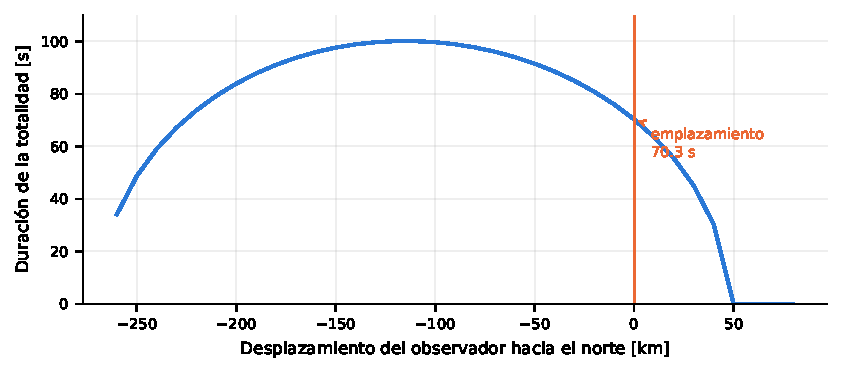
\includegraphics[width=0.8\textwidth]{../figs/fig8_path.pdf}
\caption{Duración de la totalidad en función del desplazamiento del observador
hacia el norte, calculada re-resolviendo los contactos con DE440s en cada
posición.}
\label{fig:path}
\end{figure}

\subsection{Oscurecimiento por el ocaso frente al oscurecimiento por la Luna}

Esta es la comparación que motiva buena parte del trabajo y aparece en la
figura~\ref{fig:irr} y en la tabla~\ref{tab:irr}. En el primer contacto, con el
Sol a \altCOne\textdegree{} y masa de aire \amCOne, la irradiancia normal
directa vale \dniCOne~\si{\watt\per\square\meter}. Cincuenta y cuatro minutos
más tarde, en el instante de la totalidad, esa misma irradiancia habría valido
\dniMaxNoEcl~\si{\watt\per\square\meter} \emph{sin ningún eclipse}, solo por el
descenso del Sol. Es decir, el atardecer por sí solo se lleva el
\sunsetDrop\,\% de la señal en ese intervalo, y lo hace de forma monótona y
predecible. La Luna se lleva el resto, pero lo hace en una escala de tiempo
completamente distinta: la caída final desde el 90\,\% de obscuración hasta la
totalidad ocupa \plungeMin{} minutos.

\begin{figure}[htbp]\centering
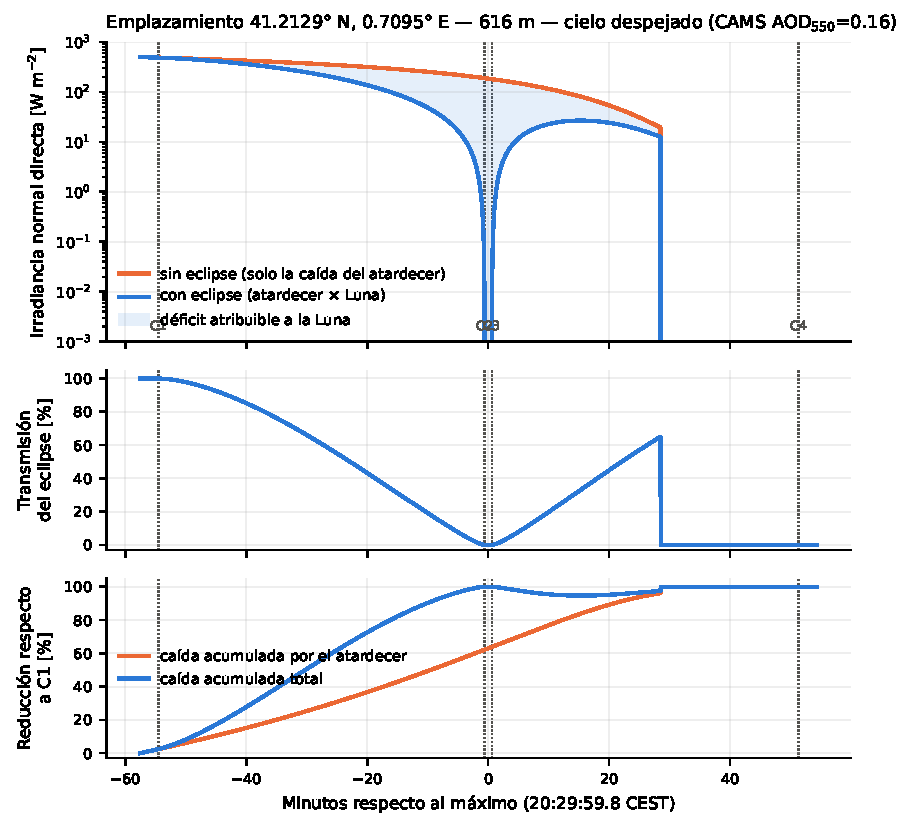
\includegraphics[width=\textwidth]{../figs/fig2_irradiance.pdf}
\caption{Panel superior: irradiancia normal directa con y sin eclipse; el área
sombreada es el déficit atribuible a la Luna. Panel central: transmisión del
eclipse. Panel inferior: reducción acumulada respecto al primer contacto,
separando la contribución del atardecer de la total.}
\label{fig:irr}
\end{figure}

\begin{table}[htbp]\centering\small
\caption{Irradiancia normal directa integrada 300--4000\,nm calculada con SPECTRL2 sobre el estado atmosférico real del día (AOD$_{550}$ = \aodFiveFiveZero, agua precipitable \pw\,cm, presión \psurf\,hPa, nubosidad \cloud\,\%).}
\label{tab:irr}
\begin{tabular}{lS[table-format=-2.2]cS[table-format=1.3]S[table-format=3.1]S[table-format=3.2]S[table-format=1.4]}
\toprule
Instante & {Altura (\textdegree)} & {Masa aire} & {Obsc.} & {DNI sin ecl.} & {DNI con ecl.} & {Transm.} \\
 & & & & {(\si{\watt\per\square\meter})} & {(\si{\watt\per\square\meter})} & \\
\midrule
C1 & 14.70 & 3.9 & 0.000 & 489.1 & 489.07 & 1.0000 \\
-1800 s & 10.17 & 5.5 & 0.338 & 374.4 & 247.68 & 0.6615 \\
-900 s & 7.44 & 7.3 & 0.666 & 286.5 & 89.51 & 0.3125 \\
-600 s & 6.53 & 8.2 & 0.785 & 254.0 & 48.74 & 0.1919 \\
-300 s & 5.64 & 9.3 & 0.905 & 220.3 & 16.92 & 0.0768 \\
-120 s & 5.10 & 10.1 & 0.976 & 199.5 & 3.38 & 0.0170 \\
-45 s & 4.88 & 10.5 & 0.999 & 190.8 & 0.15 & 0.0008 \\
máximo & 4.75 & 10.7 & 1.000 & 185.5 & 0.00 & 0.0000 \\
+45 s & 4.62 & 11.0 & 0.999 & 180.3 & 0.06 & 0.0003 \\
+120 s & 4.40 & 11.4 & 0.977 & 171.5 & 2.74 & 0.0160 \\
+600 s & 3.00 & 15.1 & 0.783 & 115.7 & 22.79 & 0.1969 \\
+1800 s & -0.22 & {--} & 0.317 & 0.0 & 0.00 & 0.0000 \\
\bottomrule
\end{tabular}
\end{table}


El oscurecimiento de limbo introduce una diferencia medible entre la fracción de
área cubierta y la fracción de flujo eliminada (figura~\ref{fig:chrom}), y como
el exponente de la ley depende de la longitud de onda, la transmisión del
eclipse es ligeramente cromática. El efecto es pequeño pero real, y reportar la
obscuración geométrica como si fuera un déficit de flujo es un error
sistemático evitable.

\begin{figure}[htbp]\centering
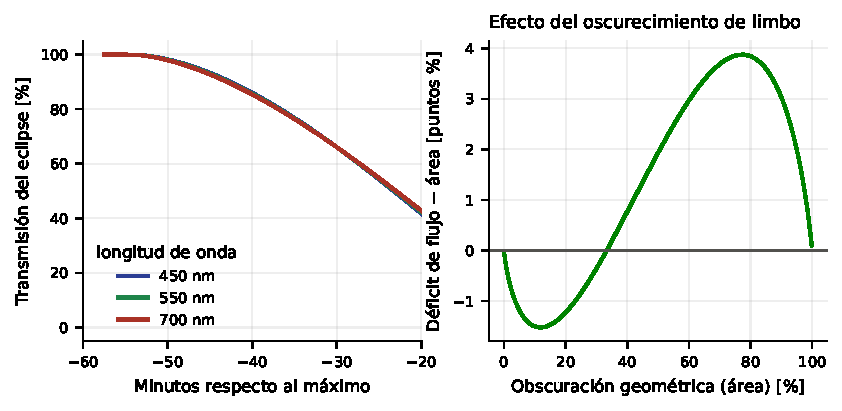
\includegraphics[width=\textwidth]{../figs/fig3_chromatic.pdf}
\caption{Izquierda: transmisión del eclipse en tres longitudes de onda durante
la fase parcial profunda. Derecha: diferencia entre el déficit de flujo a
550\,nm y la obscuración geométrica de área.}
\label{fig:chrom}
\end{figure}

\subsection{Riesgo para los sensores}

La concentración geométrica que alcanza cada configuración es
\concFSixThree soles a f/6,3 y \concFOneNine soles a f/1,9, frente a un límite
termodinámico de \concMax{} soles. El teleobjetivo cerrado, que es la
configuración que la intuición señala como peligrosa, es en realidad la más
benigna de las tres; el módulo de un teléfono a f/1,9 concentra once veces más
irradiancia que la réflex a f/6,3.

Lo que sí cambia con la focal es el tamaño de la imagen solar y la potencia
total: a 300\,mm el disco solar mide \imgDiaThreeZeroZero\,mm sobre el sensor, mientras
que a 16\,mm mide \imgDiaOneSix\,\si{\micro\meter}. La tabla~\ref{tab:focal}
recoge la irradiancia de pico, el diámetro de la imagen, la potencia total y el
incremento de temperatura local estacionario para todo el rango del objetivo, en
las condiciones del primer contacto, que son las más desfavorables de toda la
tarde.

\begin{table}[htbp]\centering\small
\caption{Plano focal en el primer contacto (Sol sin eclipsar a \altCOne\textdegree, DNI = \dniCOne~\si{\watt\per\square\meter}), con $\tau = 1$ como cota conservadora. $\Delta T$ es el incremento local estacionario en el centro de la imagen solar.}
\label{tab:focal}
\begin{tabular}{S[table-format=3.0]lS[table-format=2.2]S[table-format=1.3]S[table-format=4.1]S[table-format=1.3]}
\toprule
{Focal (mm)} & Diafragma & {$E_{\mathrm{pico}}$ (\si{\watt\per\square\centi\meter})} & {Imagen (mm)} & {Potencia (mW)} & {$\Delta T$ (K)} \\
\midrule
16 & máx. (f/3,5) & 59.42 & 0.147 & 8.0 & 0.295 \\
16 & cerrado (f/11,0) & 6.02 & 0.147 & 0.8 & 0.030 \\
16 & cerrado (f/22,0) & 1.50 & 0.147 & 0.2 & 0.007 \\
24 & máx. (f/3,8) & 51.76 & 0.220 & 15.7 & 0.385 \\
24 & cerrado (f/11,0) & 6.02 & 0.220 & 1.8 & 0.045 \\
24 & cerrado (f/22,0) & 1.50 & 0.220 & 0.5 & 0.011 \\
35 & máx. (f/4,5) & 35.95 & 0.321 & 23.2 & 0.390 \\
35 & cerrado (f/11,0) & 6.02 & 0.321 & 3.9 & 0.065 \\
35 & cerrado (f/22,0) & 1.50 & 0.321 & 1.0 & 0.016 \\
50 & máx. (f/5,1) & 28.14 & 0.459 & 37.1 & 0.436 \\
50 & cerrado (f/11,0) & 6.02 & 0.459 & 7.9 & 0.093 \\
50 & cerrado (f/22,0) & 1.50 & 0.459 & 2.0 & 0.023 \\
100 & máx. (f/5,8) & 21.64 & 0.918 & 114.2 & 0.671 \\
100 & cerrado (f/11,0) & 6.02 & 0.918 & 31.7 & 0.187 \\
100 & cerrado (f/22,0) & 1.50 & 0.918 & 7.9 & 0.047 \\
150 & máx. (f/6,3) & 18.34 & 1.377 & 217.8 & 0.853 \\
150 & cerrado (f/11,0) & 6.02 & 1.377 & 71.4 & 0.280 \\
150 & cerrado (f/22,0) & 1.50 & 1.377 & 17.9 & 0.070 \\
200 & máx. (f/6,3) & 18.34 & 1.836 & 387.1 & 1.137 \\
200 & cerrado (f/11,0) & 6.02 & 1.836 & 127.0 & 0.373 \\
200 & cerrado (f/22,0) & 1.50 & 1.836 & 31.7 & 0.093 \\
300 & máx. (f/6,3) & 18.34 & 2.754 & 871.0 & 1.706 \\
300 & cerrado (f/11,0) & 6.02 & 2.754 & 285.7 & 0.560 \\
300 & cerrado (f/22,0) & 1.50 & 2.754 & 71.4 & 0.140 \\
\bottomrule
\end{tabular}
\end{table}


El resultado central es la tabla~\ref{tab:thermal} y la figura~\ref{fig:thermal}.
En el primer contacto, la peor configuración del teleobjetivo produce
\EpkThreeZeroZero~\si{\watt\per\square\centi\meter} de irradiancia de pico y un
incremento local estacionario de \dTssThreeZeroZero\,K, alcanzado en
\tauSpotThreeZeroZero\,ms. Como referencia, la misma configuración apuntada al Sol de
mediodía en un día despejado daría \EpkThreeZeroZeroNoon~\si{\watt\per\square\centi\meter}
y \dTssThreeZeroZeroNoon\,K. En ambos casos el incremento local está dos órdenes de
magnitud por debajo de las temperaturas a las que se degradan los materiales no
silíceos del apilado, y \ordersMelt{} órdenes por debajo del punto de fusión del
silicio. Ese denominador, que una versión anterior de este trabajo dejó sin
citar, ahora puede acotarse con literatura. El elemento más frágil del apilado no
es el filtro de color sino la microlente: una microlente de fotorresina se
\emph{fabrica} fundiéndola hasta que la tensión superficial le da forma
hemisférica, de modo que su temperatura de reflujo es por construcción aquella a
la que pierde la forma, y dos trabajos independientes la sitúan entre 125 y
150\,\textdegree C \cite{hwang2009,kim2013}. La matriz de filtros de color, en
cambio, se hornea durante su fabricación a entre 150 y 250\,\textdegree C
\cite{nemoto2011}, lo que es una cota inferior de \emph{supervivencia} y no una
temperatura de degradación; una versión anterior de este texto citaba ese
intervalo en el sentido contrario. Como referencia de sistema, la hoja de datos
pública de un sensor CMOS de consumo declara 70\,\textdegree C de temperatura
máxima de operación y 125\,\textdegree C de almacenamiento como valor máximo
absoluto \cite{ov5647}.

\begin{table}[htbp]\centering\small
\caption{Incremento de temperatura local estacionario en el centro de la imagen solar, $\Delta T = qa/k$, para tres configuraciones ópticas y cuatro épocas.}
\label{tab:thermal}
\begin{tabular}{lS[table-format=3.0]S[table-format=1.3]S[table-format=1.3]S[table-format=1.4]}
\toprule
Época & {DNI (\si{\watt\per\square\meter})} & {16\,mm f/3,5 (K)} & {300\,mm f/6,3 (K)} & {f/1,9 tipo móvil (K)} \\
\midrule
mediodía solar despejado (referencia) & 900 & 0.543 & 3.140 & 0.7939 \\
C1 del eclipse (Sol a 14.7$^\circ$) & 489 & 0.295 & 1.706 & 0.4314 \\
10 min antes del máximo & 49 & 0.029 & 0.170 & 0.0430 \\
totalidad & 0 & 0.000 & 0.000 & 0.0000 \\
\bottomrule
\end{tabular}
\end{table}


\begin{figure}[htbp]\centering
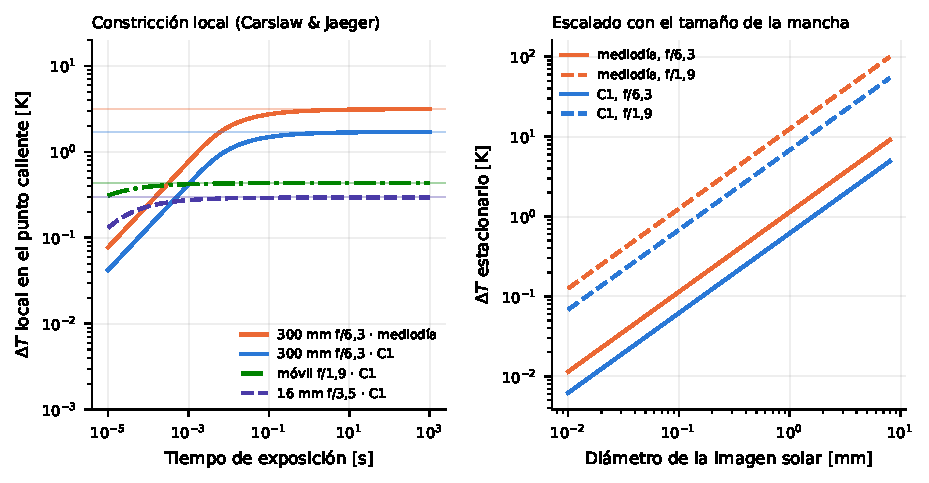
\includegraphics[width=\textwidth]{../figs/fig5_thermal.pdf}
\caption{Izquierda: evolución temporal del incremento local, con las asíntotas
en trazo fino. Derecha: escalado del incremento estacionario con el diámetro de
la imagen solar, que es la razón por la que los umbrales de daño medidos con
manchas láser micrométricas no pueden compararse directamente con una imagen
solar milimétrica.}
\label{fig:thermal}
\end{figure}

\begin{figure}[htbp]\centering
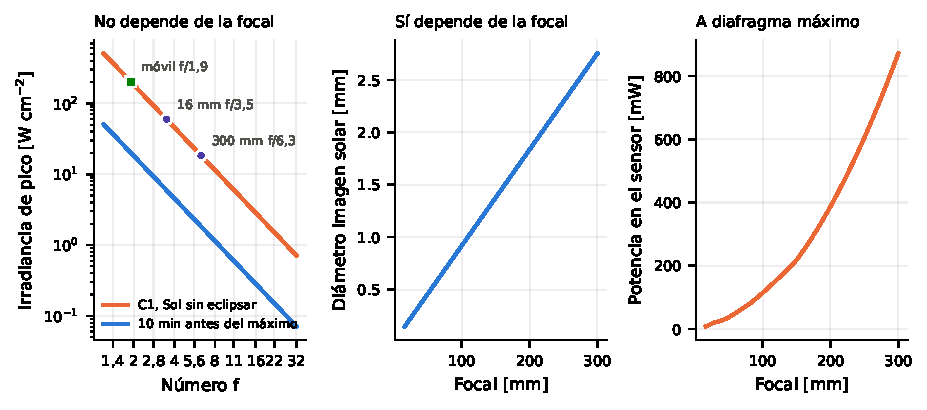
\includegraphics[width=\textwidth]{../figs/fig4_focalplane.pdf}
\caption{Izquierda: irradiancia de pico en el plano focal frente al número f,
con las configuraciones reales señaladas. Derecha: diámetro de la imagen solar
y potencia total frente a la focal, a diafragma máximo del objetivo.}
\label{fig:focal}
\end{figure}

El teléfono merece un párrafo propio, porque es el dispositivo con el que más
gente apuntará al Sol esa tarde y el que la ecuación~\eqref{eq:focal} señala
como el más expuesto en términos de irradiancia. La tabla~\ref{tab:phone} pone
sus tres módulos en la misma escala que la réflex. El resultado es que la
ventaja aparente del teleobjetivo de la réflex se invierte y se vuelve a
invertir: los módulos del teléfono concentran más vatios por centímetro cuadrado
por ser mucho más luminosos, pero su focal real es de milímetros, así que la
imagen solar mide entre diecisiete y sesenta y cuatro micrómetros y el
calentamiento local queda un factor \phoneRatio{} por debajo del de la réflex, y
entre dos y tres órdenes de magnitud por debajo de las temperaturas de
degradación genéricas discutidas más arriba. La potencia total que entra por sus diminutas pupilas de entrada
es de unos pocos milivatios. Apuntar el teléfono al Sol parcialmente eclipsado
esa tarde no supone riesgo térmico para el módulo.

\begin{table}[htbp]\centering\small
\caption{Los tres módulos traseros del Xiaomi 13T Pro en las condiciones del primer contacto. La focal real se deduce de la equivalente y del formato del sensor; la derivación se detalla en \texttt{data/hardware.json}. Pese a ser ópticas mucho más luminosas que el teleobjetivo de la réflex, la imagen solar es de decenas de micrómetros y el calentamiento local resulta un factor cuatro menor que el de la réflex, y dos o tres órdenes de magnitud por debajo de las temperaturas de degradación de sus materiales.}
\label{tab:phone}
\begin{tabular}{lS[table-format=2.1]S[table-format=1.2]S[table-format=1.2]S[table-format=3.0]S[table-format=1.3]S[table-format=1.4]}
\toprule
Módulo & {Equiv. (mm)} & {Real (mm)} & {$N$} & {Imagen (\si{\micro\meter})} & {Potencia (mW)} & {$\Delta T$ (K)} \\
\midrule
ultra gran angular & 15.0 & 1.81 & 2.20 & 17 & 0.260 & 0.0844 \\
principal & 24.0 & 6.93 & 1.90 & 64 & 5.110 & 0.4333 \\
teleobjetivo & 50.0 & 6.42 & 1.90 & 59 & 4.386 & 0.4014 \\
\bottomrule
\end{tabular}
\end{table}


\subsection{Contraste con un umbral de daño publicado}

Hasta aquí el argumento ha sido de temperatura. Existe además un umbral de daño
\emph{medido}, y la sección de métodos prometía una forma de compararlo que este
trabajo no llegaba a ejecutar. Schwarz y colaboradores \cite{schwarz2017}
midieron el umbral de daño de sensores de imagen bajo láser continuo de 532\,nm,
con exposiciones de 0,25 a 10\,s y una mancha efectiva de 9,08\,\si{\micro\meter}
de radio. Para un CMOS monocromo el umbral a 10\,s es de
49\,\si{\kilo\watt\per\square\centi\meter}, y el daño correspondiente es una
pérdida permanente de sensibilidad de los píxeles iluminados de al menos un
10\,\%, no píxeles muertos ni destrucción: el daño en línea en el mismo
dispositivo exige 196\,\si{\kilo\watt\per\square\centi\meter}. Es el único
umbral en onda continua para un sensor de silicio que se ha localizado publicado
junto con su tamaño de mancha, condición sin la cual el número no es utilizable.

La tabla~\ref{tab:threshold} lo compara con las configuraciones de este trabajo
bajo las dos hipótesis que acotan el mecanismo. Si el daño lo gobierna la
conducción en el silicio, el producto $qa$ es el invariante y el umbral cae como
$1/a$, de modo que para la imagen solar milimétrica del teleobjetivo baja hasta
\threshA~\si{\watt\per\square\centi\meter}: el margen en el primer contacto es
entonces de \marginA{}. Si en cambio lo gobierna la absorción en una capa fina
de baja conductividad, que es lo que sugieren las dos únicas fuentes que
describen cualitativamente el mecanismo en onda continua \cite{yoon2016,kim2015}
al señalar que el filtro de color falla antes que el silicio, el umbral no
depende del tamaño de la mancha y el margen sube a \marginB{}. La hipótesis
conservadora es la primera, y aun así deja un factor \marginA{} en el momento
más desfavorable de la tarde.

\begin{table}[htbp]\centering\small
\caption{Irradiancia de pico frente al único umbral de daño en onda continua publicado para un sensor de silicio con su tamaño de mancha, 49\,\si{\kilo\watt\per\square\centi\meter} sobre una mancha efectiva de 9,08\,\si{\micro\meter} de radio. La hipótesis A supone que el daño lo gobierna la conducción en el silicio, de modo que el umbral reescala como $1/a$ y baja mucho para una imagen solar milimétrica; la hipótesis B supone que lo gobierna la absorción en una capa fina de baja conductividad, en cuyo caso el umbral no depende del tamaño de la mancha. A es la conservadora.}
\label{tab:threshold}
\begin{tabular}{lS[table-format=3.1]S[table-format=4.0]S[table-format=4.0]S[table-format=5.0]}
\toprule
Configuración & {$E_{\mathrm{pico}}$} & {Umbral A} & {Margen A} & {Margen B} \\
 & \multicolumn{2}{c}{(\si{\watt\per\square\centi\meter})} & & \\
\midrule
Tamron 300\,mm f/6,3, C1 del eclipse & 18.3 & 323 & 18 & 2672 \\
Tamron 16\,mm f/3,5, C1 del eclipse & 59.4 & 6059 & 102 & 825 \\
móvil f/1,9, C1 del eclipse & 201.6 & 13989 & 69 & 243 \\
Tamron 300\,mm f/6,3, mediodía & 33.7 & 323 & 10 & 1452 \\
300\,mm f/2,8, mediodía & 170.9 & 323 & 2 & 287 \\
600\,mm f/4, mediodía & 83.7 & 162 & 2 & 585 \\
\bottomrule
\end{tabular}
\end{table}


Merece la pena mirar la última fila de esa tabla, porque es donde el ejercicio
deja de ser tranquilizador. Un teleobjetivo de 300\,mm a f/2,8 apuntado al Sol
de mediodía se queda en un margen de \marginFast{} bajo la hipótesis
conservadora. Los objetivos rápidos y largos que se usan precisamente para
fotografiar el Sol son los que se acercan al umbral; el zoom lento del observador
a 4,75\textdegree{} de altura estaba dos órdenes de magnitud más lejos de él. La
advertencia general está justificada, y a la vez el caso concreto de esta tarde
no lo estaba.

Dos cautelas sobre esta comparación. La primera es que Schwarz y colaboradores
midieron un sensor de visión artificial de 2010 con píxeles de
6\,\si{\micro\meter}, no un sensor de consumo moderno, y no se ha localizado
ninguna medida equivalente para éstos. La segunda es que sus umbrales en onda
continua \emph{disminuyen} con el tiempo de exposición, de 85 a
49\,\si{\kilo\watt\per\square\centi\meter} entre 0,25 y 10\,s, cuando una mancha
de 25\,\si{\micro\meter} en silicio alcanza su estado estacionario en microsegundos.
Esa dependencia temporal demuestra que el daño no lo gobierna únicamente el
estado estacionario local, de modo que ninguna de las dos hipótesis es exacta y
la horquilla debe leerse como tal. No se ha localizado ninguna segunda medida
absoluta en onda continua con la que contrastar: la que existe declara
expresamente que sus intensidades se publican en valor relativo por motivos de
seguridad \cite{yoon2016}.

En cuanto al tiempo máximo de exposición, que es la pregunta explícita que
motivó este trabajo, la respuesta tiene dos partes. La componente local no
impone ningún límite temporal, porque satura en milisegundos por debajo de
cualquier umbral. La componente que sí crece con el tiempo es el calentamiento
global del conjunto sensor-encapsulado por la potencia total absorbida, que a
300\,mm y f/6,3 en el primer contacto vale \PglobThreeZeroZero\,mW, frente a
\PglobOneSix\,mW a 16\,mm y f/3,5. Con resistencias térmicas plausibles para una
cámara compacta, de entre 10 y 50~\si{\kelvin\per\watt}, el teleobjetivo
produciría un incremento estacionario de entre \dTglobThreeZeroZeroLo\,K y
\dTglobThreeZeroZeroHi\,K tras varios minutos de apuntado continuo. Ese
intervalo es paramétrico y no una predicción: no se localizó un valor publicado
de resistencia térmica para esta cámara, y se declara como tal.
Ese rango queda dentro de la temperatura de operación típica de un CMOS de
consumo, aunque no se localizó una especificación para esta cámara concreta; en
todo caso degrada la imagen por aumento de corriente de oscuridad, y es la razón
práctica para no dejar la cámara apuntando al Sol entre disparos. Durante la totalidad la cuestión desaparece por completo: el cálculo da una
obscuración de 1,0000 entre el segundo y el tercer contacto, es decir, el haz
fotosférico directo es cero por construcción, y con él desaparece la única
fuente de calentamiento que este trabajo modela. La corona, mucho más débil, no
se modela aquí; que la totalidad puede observarse sin filtro es precisamente la
recomendación de la American Astronomical Society \cite{aas}, que indica
retirar el filtro \emph{solo} cuando la Luna cubre por completo el disco
brillante.

Hay, sin embargo, un límite de exposición que sí es real y que la pregunta
original no anticipaba: el arrastre de la imagen por la rotación terrestre. En
el instante de la totalidad el Sol se desplaza sobre el cielo a
\driftRate\,segundos de arco por segundo, valor obtenido diferenciando la
efeméride y no de una regla aproximada. Sobre el sensor de la réflex eso
significa que a 300\,mm la imagen recorre un píxel en \driftThreeZeroZero\,s y a
16\,mm en \driftOneSix\,s (tabla~\ref{tab:drift}). Con la cámara sobre trípode
fijo, ese es el límite que manda durante la totalidad, no el térmico, y es
además la restricción que decide qué se puede hacer con la corona y con una
eventual Perseida en el mismo encuadre.

\begin{table}[htbp]\centering\small
\caption{Límite de exposición impuesto por el arrastre de la imagen durante la totalidad, para el sensor de la EOS 200D (paso de píxel 3,72\,\si{\micro\meter}). La velocidad angular aparente del Sol en ese instante, 14.31''/s, se obtiene diferenciando la efeméride, no de una regla aproximada. Con la cámara sobre trípode fijo este es el límite que manda, no el térmico.}
\label{tab:drift}
\begin{tabular}{S[table-format=3.0]S[table-format=2.2]S[table-format=1.2]S[table-format=2.2]}
\toprule
{Focal (mm)} & {Escala (''/px)} & {1 px (s)} & {3 px (s)} \\
 & & \multicolumn{2}{c}{Exposición máxima sin arrastre} \\
\midrule
16 & 47.91 & 3.35 & 10.05 \\
24 & 31.94 & 2.23 & 6.70 \\
35 & 21.90 & 1.53 & 4.59 \\
50 & 15.33 & 1.07 & 3.22 \\
100 & 7.67 & 0.54 & 1.61 \\
200 & 3.83 & 0.27 & 0.80 \\
300 & 2.56 & 0.18 & 0.54 \\
\bottomrule
\end{tabular}
\end{table}


\subsection{Alcance del modelo: lo que no cubre}

Todo lo anterior describe el \emph{sensor}. En una réflex el Sol rara vez está
sobre el sensor: con el espejo bajado, que es la posición de encuadre por el
visor óptico, la imagen solar se forma sobre la \emph{pantalla de enfoque} y de
ahí sale hacia el ocular; con el espejo levantado y el obturador cerrado, cae
sobre la \emph{cortinilla}. Ninguna de las dos piezas se comporta como el
silicio. Una cortinilla tiene decenas de micrómetros de espesor y no descansa
sobre ningún sumidero, y una pantalla de enfoque es un plástico moldeado con una
conductividad térmica tres órdenes de magnitud menor que la del silicio. En el
mismo peor caso de la tarde y con la misma potencia de \PglobThreeZeroZero\,mW,
el modelo de placa delgada da del orden de \dTshutterAl\,K para una cortinilla
metálica de 25\,\si{\micro\meter}, y valores tan altos que el modelo pierde
sentido físico para una cortinilla de composite o para una pantalla de acrílico.
Esas cifras no deben leerse como predicciones cuantitativas, porque el modelo
ignora pérdidas por radiación y convección y no contempla cambio de fase; lo que
sí indican sin ambigüedad es el orden relativo: de las tres superficies sobre las
que puede caer la imagen solar en una réflex, el sensor es con diferencia la más
protegida, por estar respaldado por silicio y por un encapsulado. La afirmación
de que en la práctica lo que se quema es la cortinilla o la pantalla de enfoque
circula ampliamente entre fotógrafos, y una búsqueda dirigida no ha localizado
para ella ninguna fuente revisada por pares. Más aún: las fuentes autorizadas
que sí hablan de daño a la cámara apuntan al sensor. La guía de fotografía solar
de Nikon, firmada por Espenak, dice literalmente que el filtro solar hace falta
«para evitar dañar el sensor de imagen de la cámara» \cite{nikonespenak}, y la
guía de seguridad de la NASA no menciona daño interno a la cámara en absoluto:
todas sus advertencias sobre óptica se refieren al ojo \cite{nasasafety}. La
conclusión de esta subsección se sostiene por tanto sobre el cálculo de placa
delgada de este trabajo y no sobre la literatura, y así debe leerse.

A esto se añade el riesgo que no es de hardware. El visor óptico entrega al ojo
la imagen concentrada por el objetivo, y la American Astronomical Society
advierte expresamente contra mirar el Sol sin eclipsar o parcialmente eclipsado
a través de una cámara, telescopio o prismáticos sin filtro \cite{aas}. Este
trabajo no modela esa vía, y la ausencia de un cálculo no debe leerse como
ausencia de riesgo: es, con diferencia, el peligro más serio de todo el montaje.

La consecuencia operativa es que la recomendación de usar filtro solar delantero
durante las fases parciales se mantiene íntegra, y que su justificación no es la
que uno esperaría. No es el sensor. Son la cortinilla, la pantalla de enfoque y
el ojo del observador.

Conviene subrayar que la conclusión térmica es específica de la altura solar de
este eclipse y de la óptica considerada. No debe extrapolarse a un eclipse con el Sol
alto, ni a teleobjetivos más luminosos, ni al Sol sin eclipsar en condiciones
normales.

\subsection{Los últimos segundos: el anillo de diamante}

Entre las curvas suaves de las secciones anteriores y lo que realmente se ve por
el visor hay un tramo que merece resolverse aparte, porque ocurre en menos
tiempo del que dura pulsar el disparador. La tabla~\ref{tab:diamond} y la
figura~\ref{fig:diamond} siguen el creciente residual de fotosfera durante el
último minuto antes del segundo contacto, con paso de cinco centésimas de
segundo.

Diez segundos antes de C2 queda todavía una milésima del área del disco, pero
solo tres diezmilésimas del flujo. La diferencia entre ambas columnas es el
oscurecimiento de limbo actuando en su régimen extremo: lo último que la Luna
tapa es el borde del disco, que es la parte más oscura, de modo que el flujo se
apaga sistemáticamente por delante del área. En el último segundo el flujo
residual cae con un tiempo de $e$-folding de \efold\,s, es decir que se divide
por diez cada seis décimas de segundo. Esa es la escala temporal del anillo de
diamante, y explica por qué una horquilla de exposición fina alrededor del
segundo contacto captura imágenes tan distintas con diferencias de medio
segundo.

Una advertencia sobre este cálculo en concreto. Todo el trabajo emplea el limbo
lunar medio, una circunferencia. El limbo real tiene montañas de varios
kilómetros, y son ellas las que rompen el creciente final en las perlas de
Baily. La curva calculada es por tanto la envolvente lisa de un fenómeno que en
realidad es escalonado, y los instantes de contacto reales pueden desplazarse
uno o dos segundos respecto a los tabulados. Modelar eso exigiría un perfil de
limbo, que este trabajo no incorpora.

\begin{table}[htbp]\centering\small
\caption{Los últimos segundos de fotosfera antes del segundo contacto, en fracción del disco sin eclipsar. El flujo se extingue más deprisa que el área porque lo último que queda es limbo, que es la parte oscura del disco. Calculado con el limbo lunar MEDIO: las montañas reales de la Luna rompen el creciente en las perlas de Baily y hacen que la curva real sea escalonada, no lisa.}
\label{tab:diamond}
\begin{tabular}{S[table-format=-2.1]S[table-format=1.2e2]S[table-format=1.2e2]S[table-format=1.2]}
\toprule
{$t-t_{C2}$ (s)} & {Área restante} & {Flujo restante} & {Flujo/Área} \\
\midrule
-60.0 & 1.46e-02 & 6.83e-03 & 0.47 \\
-30.0 & 5.47e-03 & 2.11e-03 & 0.39 \\
-10.0 & 1.06e-03 & 3.05e-04 & 0.29 \\
-5.0 & 3.71e-04 & 8.90e-05 & 0.24 \\
-2.0 & 9.32e-05 & 1.77e-05 & 0.19 \\
-1.0 & 3.28e-05 & 5.21e-06 & 0.16 \\
-0.5 & 1.16e-05 & 1.54e-06 & 0.13 \\
-0.2 & 2.93e-06 & 3.09e-07 & 0.11 \\
-0.1 & 1.04e-06 & 9.22e-08 & 0.09 \\
\bottomrule
\end{tabular}
\end{table}


\begin{figure}[htbp]\centering
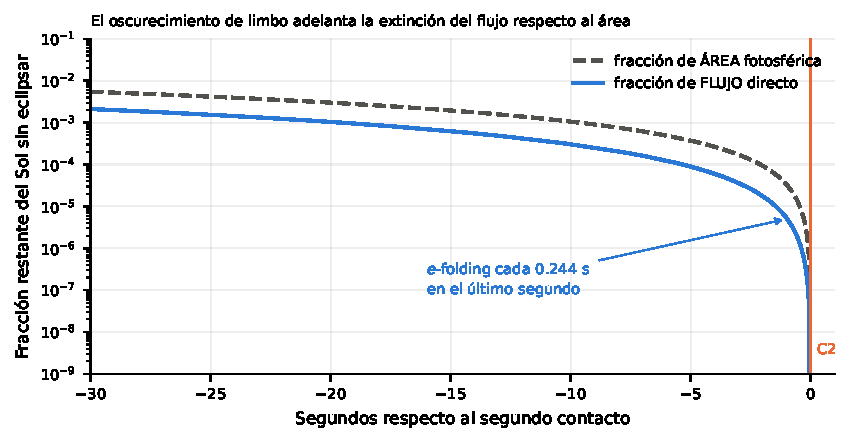
\includegraphics[width=0.82\textwidth]{../figs/fig10_diamondring.pdf}
\caption{Fracción de área y de flujo fotosférico que sobrevive en los últimos
treinta segundos antes del segundo contacto. Las dos curvas divergen porque lo
último que queda es limbo oscurecido.}
\label{fig:diamond}
\end{figure}

\subsection{Riesgo para el ojo}

Aquí la conclusión se invierte. La tabla~\ref{tab:eye} y la
figura~\ref{fig:eye} muestran la irradiancia eficaz de luz azul y el tiempo
máximo de fijación que ICNIRP admite.

\begin{table}[htbp]\centering\small
\caption{Riesgo ocular según ICNIRP 2013. $E_B$ es la irradiancia corneal ponderada con $B(\lambda)$. El tiempo de fijación es $100/E_B$ segundos mientras $E_B > 1$~\si{\watt\per\square\meter}, e ilimitado por debajo de ese valor.}
\label{tab:eye}
\begin{tabular}{lS[table-format=-2.2]S[table-format=1.3]S[table-format=2.3]S[table-format=2.3]rr}
\toprule
Instante & {Altura (\textdegree)} & {Obsc.} & {$E_B$ sin ecl.} & {$E_B$ con ecl.} & Fijación sin ecl. & Fijación con ecl. \\
 & & & {(\si{\watt\per\square\meter})} & {(\si{\watt\per\square\meter})} & (s) & (s) \\
\midrule
C1 & 14.70 & 0.000 & 24.014 & 24.014 & 4.2 & 4.2 \\
-2400 s & 12.01 & 0.157 & 17.195 & 14.790 & 5.8 & 6.8 \\
-1800 s & 10.17 & 0.338 & 12.466 & 8.244 & 8.0 & 12 \\
-1200 s & 8.34 & 0.551 & 8.010 & 3.357 & 12 & 30 \\
-900 s & 7.44 & 0.666 & 6.005 & 1.756 & 17 & 57 \\
-600 s & 6.53 & 0.785 & 4.227 & 0.717 & 24 & $\infty$ \\
-300 s & 5.64 & 0.905 & 2.735 & 0.165 & 37 & $\infty$ \\
-120 s & 5.10 & 0.976 & 1.998 & 0.022 & 50 & $\infty$ \\
máximo & 4.75 & 1.000 & 1.577 & 0.000 & 63 & $\infty$ \\
+300 s & 3.87 & 0.906 & 0.775 & 0.047 & $\infty$ & $\infty$ \\
+900 s & 2.15 & 0.661 & 0.086 & 0.026 & $\infty$ & $\infty$ \\
\bottomrule
\end{tabular}
\end{table}


En el primer contacto, con el Sol a \altCOne\textdegree{} y todavía sin
eclipsar, la irradiancia eficaz de luz azul vale \EBCOne~\si{\watt\per\square\meter},
veinticuatro veces el límite de exposición prolongada, y el tiempo máximo de
fijación es de \stareCOne\,s. El límite térmico retiniano, por su parte, también se
supera: la razón entre la radiancia ponderada y el límite vale
\thermRatioCOne, un \thermExcessCOne\,\% por encima, y alcanza \thermRatioPeak{}
poco antes del primer contacto. A diferencia del fotoquímico, este cociente no
se desploma con la obscuración, porque la radiancia del creciente no cambia:
decae solo en la medida en que lo hace la transmisión atmosférica y en que el
creciente se estrecha.

Lo relevante para quien vaya a observar es lo que ocurre después. En el instante
de la totalidad, el Sol \emph{sin eclipsar} a \altMax\textdegree{} habría dado
\EBnoEclMax~\si{\watt\per\square\meter}, todavía por encima del límite, con un
tiempo de fijación de \stareNoEclMax\,s. Es decir: incluso con el Sol a menos de
cinco grados y once masas de aire de atmósfera por delante, mirarlo fijamente
más de un minuto excede la dosis fotoquímica admisible. La creencia de que el
Sol bajo es inofensivo porque no deslumbra es precisamente el mecanismo del
daño: la respuesta de aversión desaparece mucho antes que el peligro.

Hay un supuesto en todo lo anterior que conviene sacar a la luz, porque va en la
dirección insegura. La forma en irradiancia de los límites ICNIRP no elimina la
pupila del problema: la propia guía indica que el límite fotoquímico
\emph{se derivó suponiendo un diámetro de pupila de aproximadamente 3\,mm}. La
dosis retiniana escala con el área pupilar, de modo que un observador cuya
pupila se haya abierto hasta $d$ milímetros recibe $(d/3)^2$ veces la dosis que
el límite presupone. Y eso es exactamente lo que ocurre aquí, porque el cielo se
oscurece según avanza el eclipse. Para el Sol sin eclipsar en el instante de la
totalidad, el tiempo máximo de fijación pasa de \stareNoEclMaxPThree\,s con la
pupila nominal de 3\,mm a \stareNoEclMaxPFive\,s con 5\,mm y
\stareNoEclMaxPSeven\,s con 7\,mm. En el primer contacto pasa de
\stareCOnePThree\,s a \stareCOnePSeven\,s.

Ahora bien, cuál de esas cifras es la realista merece una discusión que no
conviene despachar, porque el argumento tiene dos direcciones. El diámetro
pupilar no lo fija el brillo del cielo sino la iluminancia retiniana, y quien
mira al Sol está fijando precisamente el creciente de fotosfera, cuyo brillo
\emph{de superficie} el eclipse no altera en absoluto: la Luna quita área, no
radiancia. Mientras quede fotosfera visible, el estímulo que gobierna la
constricción sigue siendo deslumbrante y cabe esperar una pupila próxima a la
nominal de 3\,mm. Contra eso juega que la iluminancia retiniana total sí cae con
la obscuración, que el campo circundante se oscurece de forma acusada en los
últimos minutos, y que la constricción pupilar tiene una constante de tiempo de
segundos, de modo que en la reaparición de la fotosfera tras el tercer contacto
la pupila viene francamente dilatada y tarda en cerrarse.

De ahí que este trabajo reporte las tres cifras en lugar de elegir una. Para las
fases parciales tempranas, con el disco todavía cegador, la columna de 3\,mm es
probablemente la representativa. Para el tercer contacto, con el ojo recién
salido de la totalidad, la de 7\,mm es la que hay que respetar, y es también la
que sustenta la regla operativa de reponer el filtro \emph{antes} de que el Sol
reaparezca en lugar de en el momento en que reaparece. No se ha localizado una
medida publicada del diámetro pupilar de observadores durante las fases
parciales de un eclipse, de modo que la elección se declara como acotación y no
como dato.

Combinando el descenso del Sol con la obscuración creciente, el conjunto
Sol-eclipse deja de superar los límites ICNIRP a partir de \unlimitedFromPThree{} minutos respecto al máximo con
pupila de 3\,mm, pero solo a partir de \unlimitedFromPSeven{} minutos si la
pupila se ha dilatado a 7\,mm. Esto no es una autorización para mirar sin filtro. Los límites
ICNIRP son límites de exposición ocupacional con un factor de reducción
declarado de al menos dos frente a los umbrales de daño, no garantías de
confort ni de ausencia de efectos; y el margen desaparece por completo en el
tercer contacto, cuando reaparece la fotosfera de golpe con el ojo ya adaptado a
la oscuridad y la pupila dilatada, que es el escenario clásico de retinopatía
solar. La recomendación operativa no cambia y coincide con la de la American
Astronomical Society \cite{aas}: filtro certificado ISO 12312-2 salvo durante
los \totalityDur\,s de totalidad, retirándolo \emph{solo} cuando la Luna cubre
por completo el disco brillante y reponiéndolo \emph{en cuanto} el Sol brillante
empiece a reaparecer. La misma fuente advierte expresamente contra mirar el Sol
sin eclipsar o parcialmente eclipsado a través de una cámara, telescopio o
prismáticos sin filtro, que es exactamente la configuración analizada en la
sección anterior desde el punto de vista del sensor.

\begin{figure}[htbp]\centering
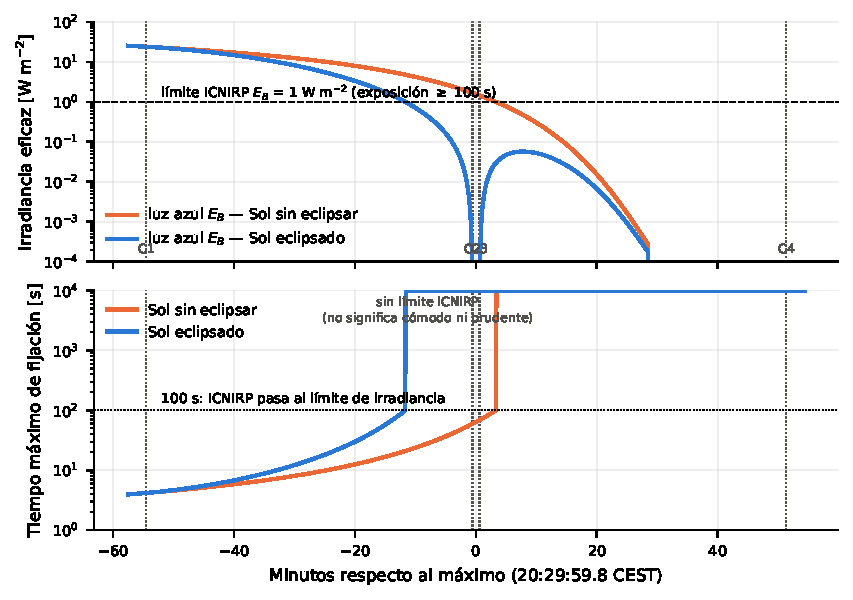
\includegraphics[width=\textwidth]{../figs/fig6_eye.pdf}
\caption{Arriba: irradiancia eficaz de luz azul con y sin eclipse, frente al
límite ICNIRP de exposición prolongada. Abajo: tiempo máximo de fijación
admisible.}
\label{fig:eye}
\end{figure}

\subsection{Perseidas durante la totalidad}

En el instante de la totalidad el radiante de las Perseidas está a solo
\radiantAlt\textdegree{} de altura, y la longitud solar es \lamSun\textdegree,
unas ocho horas antes del nodo del máximo. El radiante está a
\radiantSunSep\textdegree{} del Sol eclipsado, de modo que ningún encuadre
razonable contiene ambos. La tabla~\ref{tab:per} y la figura~\ref{fig:per}
recogen la probabilidad de que aparezca al menos una Perseida en el encuadre
durante los \totalityDur\,s de totalidad. Incluso adoptando el ZHR de 100 del
máximo, que es una cota superior generosa dado que el propio calendario del IMO
advierte que la actividad de fondo en 2026 será notablemente inferior, la
probabilidad con un gran angular de 16\,mm es del \pPerseidOneSix\,\% con
magnitud límite 3, y no supera el \pPerseidMax\,\% en ninguna combinación del
barrido.

\begin{table}[htbp]\centering\small
\caption{Probabilidad de al menos una Perseida en el encuadre durante la totalidad, formato APS-C, magnitud límite asumida 3. Los cuatro escenarios de ZHR son un barrido de sensibilidad, no una predicción.}
\label{tab:per}
\begin{tabular}{S[table-format=3.0]lS[table-format=1.4]S[table-format=1.3]S[table-format=1.3]S[table-format=1.3]S[table-format=1.3]}
\toprule
{Focal (mm)} & Campo (\textdegree) & {$\Omega$ (sr)} & {ZHR 10} & {ZHR 20} & {ZHR 43} & {ZHR 100} \\
 & & & \multicolumn{4}{c}{Probabilidad (\%)} \\
\midrule
16 & 69.7 $\times$ 49.9 & 0.9750 & 0.031 & 0.061 & 0.132 & 0.306 \\
24 & 49.8 $\times$ 34.5 & 0.5009 & 0.016 & 0.031 & 0.068 & 0.157 \\
35 & 35.3 $\times$ 24.0 & 0.2529 & 0.008 & 0.016 & 0.034 & 0.079 \\
50 & 25.1 $\times$ 16.9 & 0.1283 & 0.004 & 0.008 & 0.017 & 0.040 \\
100 & 12.7 $\times$ 8.5 & 0.0329 & 0.001 & 0.002 & 0.004 & 0.010 \\
200 & 6.4 $\times$ 4.3 & 0.0083 & 0.000 & 0.001 & 0.001 & 0.003 \\
300 & 4.3 $\times$ 2.8 & 0.0037 & 0.000 & 0.000 & 0.000 & 0.001 \\
\bottomrule
\end{tabular}
\end{table}


\begin{figure}[htbp]\centering
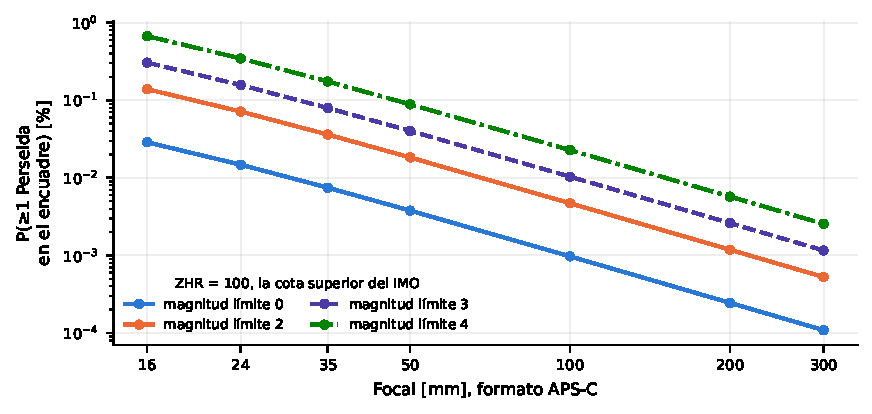
\includegraphics[width=0.8\textwidth]{../figs/fig9_perseids.pdf}
\caption{Probabilidad de captura de una Perseida durante la totalidad frente a
la focal, para cuatro magnitudes límite asumidas.}
\label{fig:per}
\end{figure}

La conclusión es que la fotografía combinada de corona y Perseida es, en la
práctica, inalcanzable en esta ventana. Merece la pena señalar dónde sí es
alcanzable: la misma noche, entre las 22:46\,CEST en que comienza la noche
astronómica y el amanecer, con el radiante subiendo y sin Luna, la ventana es de
horas en lugar de un minuto y la probabilidad se vuelve alta.

\subsection{Contraste con las fotografías de la observación}
\label{sec:fotos}

El eclipse ocurrió y el observador fotografió las fases parciales y la
totalidad. Sus 23 archivos, doce JPEG y once CR2 de una Canon EOS 200D con el
Tamron 16--300, permiten contrastar parte de lo anterior con medidas en lugar de
con modelos. El análisis completo está en \texttt{docs/PHOTOS.md}; aquí van las
tres cosas que decide.

\textbf{La escala de placa se confirma al 0,1\,\%.} El paso de píxel de la hoja
de Canon, la focal de 300\,mm del EXIF y el radio solar aparente de la efeméride
predicen un radio de 86,4 píxeles en las miniaturas analizadas. El ajuste de
circunferencia sobre el fotograma mejor condicionado da 86,5. Ninguno de los tres
ingredientes se ajustó a los datos, de modo que la cadena óptica queda validada
de extremo a extremo.

\textbf{El observador disparó a f/40}, el diafragma mínimo del objetivo a
300\,mm, con 1/4000\,s e ISO 100. La irradiancia en el plano focal cae con el
cuadrado del número f, así que la configuración real estuvo cuarenta veces por
debajo del peor caso de la tabla~\ref{tab:threshold}, que ya dejaba un factor
\marginA{} de margen. Las dos horas de fase parcial transcurrieron sin
acercarse al umbral.

\textbf{No hay un solo píxel caliente persistente.} Comparando dos tomas a
ISO 12800 separadas cinco segundos durante la totalidad, 196 píxeles superan
50\,$\sigma$ en cada una y ninguno lo hace en las dos a la vez: son ruido de
disparo, no defectos fijos. A ISO 100 aparece un píxel entre 24\,216\,480.

Ese último resultado exige una advertencia que no conviene ahorrar. No existe
fotograma anterior al eclipse, así que se trata de un recuento absoluto y no de
un cambio. Y sobre todo, el modo de daño que Schwarz y colaboradores describen
para irradiación continua es una pérdida de sensibilidad que se manifiesta en
campo plano, no un píxel caliente en una toma oscura. Estas imágenes no pueden
descartarlo. El resultado es compatible con el margen calculado y no lo verifica.

Una última observación, que es un fallo del método y no del equipo: el reloj de
la cámara iba unos tres minutos adelantado. Se deduce por ordenamiento, sin
modelo fotométrico, exigiendo que la ráfaga de corona caiga dentro de la
totalidad. La consecuencia es que estas fotografías no pueden verificar los
instantes absolutos de contacto. Quien repita el ejercicio debería sincronizar la
cámara antes de salir; cuesta un minuto y convierte cada disparo en una medida
de tiempo.

\section{Discusión}

\subsection{Incertidumbres de la cadena de cálculo}

La cadena de cálculo tiene tres eslabones con incertidumbre desigual y conviene
ser explícito sobre cada uno.

La geometría es el eslabón más firme en cuanto a instantes y el más frágil en
cuanto a duración. Los contactos están determinados a mejor que un segundo por
la efeméride, pero la duración de la totalidad depende de la posición del
observador dentro de una franja que la incidencia rasante hace muy sensible, y
la horquilla entre soluciones de sombra es de unos quince segundos. Lo que sí
está firmemente establecido es que el emplazamiento está dentro de la franja con
margen: \northLimit\,km hasta el límite norte.

La irradiancia es el eslabón más débil, y conviene enseñar cuánto. A masa de
aire \amMax{} ningún modelo de cielo claro está dentro de su rango de
validación. La dispersión entre las distintas fórmulas de masa de aire es solo
del \amSpread\,\% a esta altura, de modo que ese no es el problema; el problema
son las parametrizaciones de extinción. El cálculo espectral reproduce el patrón
ASTM G173 con \gerr\,\% de error a masa de aire 1,5, pero eso no garantiza su
comportamiento a masa de aire once.

La tabla~\ref{tab:ensemble} cuantifica el asunto ejecutando tres modelos
independientes sobre la misma geometría y el mismo estado atmosférico. A masa de
aire cuatro concuerdan dentro de un 26\,\%; en el instante de la totalidad
difieren en un factor \dniMaxSpread, entre \dniMaxLow{} y
\dniMaxHigh~\si{\watt\per\square\meter}. Esa horquilla, y no el error formal de
ninguno de ellos, es la incertidumbre real.

\begin{table}[htbp]\centering\small
\caption{Tres modelos de cielo claro sobre la misma geometría y el mismo estado atmosférico. La dispersión crece de un 26\,\% a masa de aire 4 hasta un factor 3,0 a masa de aire 11, y esa dispersión es la incertidumbre real de la cadena radiométrica, no el error formal de ninguno de ellos. El paper adopta SPECTRL2, que es el más alto de los tres, porque es la elección conservadora para el riesgo ocular.}
\label{tab:ensemble}
\begin{tabular}{lS[table-format=2.2]S[table-format=2.2]S[table-format=3.1]S[table-format=3.1]S[table-format=3.1]S[table-format=1.2]}
\toprule
Instante & {Altura (\textdegree)} & {Masa aire} & {SPECTRL2} & {Bird--Hulstrom} & {Ineichen--Perez} & {Razón máx/mín} \\
 & & & \multicolumn{3}{c}{DNI sin eclipse (\si{\watt\per\square\meter})} & \\
\midrule
C1 & 14.70 & 3.9 & 489.1 & 467.1 & 389.7 & 1.26 \\
30 min antes del máximo & 10.17 & 5.5 & 374.4 & 348.6 & 252.1 & 1.49 \\
instante de la totalidad & 4.75 & 10.7 & 185.5 & 154.0 & 61.1 & 3.04 \\
\bottomrule
\end{tabular}
\end{table}


Las consecuencias son asimétricas y hay que decirlas con claridad. Para la
conclusión instrumental no cambia nada: incluso multiplicando por tres la
irradiancia más alta, el incremento local seguiría dos órdenes de magnitud por
debajo de cualquier umbral. Para la conclusión ocular sí importa. Este trabajo
adopta SPECTRL2, que es el más alto de los tres y por tanto la elección
conservadora; con el más bajo, el Sol sin eclipsar en el instante de la
totalidad quedaría en el entorno del límite fotoquímico en lugar de por encima,
y el tiempo de fijación de \stareNoEclMax\,s dejaría de ser un límite estricto.
Dicho de otro modo: la cifra concreta de segundos depende del modelo, pero el
signo de la conclusión, que el Sol bajo de esa tarde no es inocuo, se mantiene
en todo el rango, y la recomendación operativa de usar filtro certificado no
depende de ninguno de ellos.

Los valores de entrada atmosféricos son pronósticos operativos, no medidas, con
una excepción. La columna total de ozono sí es una medida: procede de la estación
411 del WOUDC en Zaragoza, un espectrofotómetro Brewer MKIV operado por AEMET a
136\,km del emplazamiento y prácticamente a la misma latitud \cite{woudc}. Sus
189 días de observación en la ventana del 8 al 16 de agosto entre 2001 y 2024 dan
$310{,}9 \pm 13{,}8$\,DU, y el conjunto de agosto completo, 630 días, da
$309{,}3 \pm 12{,}4$\,DU con un recorrido de 280 a 364. Se adopta
0,3109\,atm-cm. El interés de haberlo medido no está en el valor sino en la
comprobación de que da igual: pasar del 0,300\,atm-cm que este trabajo suponía
antes al valor observado mueve el haz directo un 0,09\,\% y la irradiancia
eficaz de luz azul un 0,03\,\%, y recorrer todo el rango histórico las mueve
menos de un 0,7\,\%. La irrelevancia del ozono queda demostrada en lugar de
afirmada. La transmitancia del
objetivo no está publicada y se sustituye por la cota conservadora $\tau = 1$.
Las dimensiones del sensor de la réflex, 22,3 por 14,9\,mm, proceden de la hoja
de especificaciones de producto de Canon (copia servida por una CDN de terceros), de la que resulta un paso de píxel de
3,72\,\si{\micro\meter}; solo intervienen en la fracción de encuadre ocupada por
la imagen solar y en el campo de visión usado para las Perseidas, no en ninguna
conclusión de seguridad.

Finalmente, el modelo térmico local supone conducción en un sólido semiinfinito
de silicio, y esa idealización deja de ser válida antes de lo que parece. La
imagen solar del teleobjetivo mide \imgDiaThreeZeroZero\,mm de diámetro, mucho
más que el espesor de un dado adelgazado, de unas décimas de milímetro; el
frente térmico alcanza esa profundidad en un milisegundo, es decir mucho antes
de que la solución semiinfinita llegue a su asíntota. Hay entonces tres regímenes
y conviene dar los tres en lugar de un supuesto intervalo:
con un buen sumidero por detrás el calor atraviesa el dado casi en una dimensión
y el incremento es $q\,e/k = \dTonedThreeZeroZero$\,K para $e = 0{,}3$\,mm; la
solución semiinfinita da \dTssThreeZeroZero\,K; y si la cara trasera es
adiabática y el calor debe extenderse lateralmente dentro de una placa de
0,3\,mm hasta el borde del sensor, la resistencia de expansión
$\ln(b/a)/(2\pi k e)$ eleva el incremento hasta \dTworstThreeZeroZero\,K. Es
este último, y no el semiinfinito, el peor caso defendible. Sigue estando muy
por debajo de cualquier temperatura de degradación, pero el margen es de un
factor del orden de treinta, no de dos órdenes de magnitud.

\section{Conclusiones}

El emplazamiento es válido: está dentro de la franja de totalidad con
\perpLimit\,km de margen perpendicular hasta el límite norte, y su horizonte real hacia el
poniente está despejado con \clearance\textdegree{} de holgura. La totalidad
duró \totalityDur\,s alrededor de las \localMax\,CEST, valor que dos soluciones
de sombra independientes acotan en 1,4\,s.

Para el \emph{sensor} de la réflex con el Tamron 16--300 y para los tres módulos
del teléfono no hay riesgo térmico apreciable a esta altura solar en ninguna
combinación de focal y diafragma: incluso en la idealización más desfavorable el
incremento local se queda en \dTworstThreeZeroZero\,K, y durante la totalidad el
haz directo es cero. Esa conclusión no se extiende al resto de la cámara. La
cortinilla del obturador y la pantalla de enfoque son piezas delgadas y mal
refrigeradas sobre las que la misma imagen solar cae durante el encuadre y entre
disparos, y a las que el modelo asigna temperaturas muy superiores. Por eso
el filtro solar delantero sigue siendo necesario durante toda la fase parcial, y
por eso conviene encuadrar en visión en directo y no por el visor óptico, que
entrega al ojo el haz concentrado por el objetivo.

Para el ojo, la conclusión es la opuesta y debe tomarse en serio. El Sol bajo de
esa tarde sigue superando el límite fotoquímico de ICNIRP hasta
\unlimitedFromPSeven{} minutos antes de la totalidad si se toma la pupila
dilatada, que es la hipótesis que hay que respetar en el tercer contacto, y lo hace sin producir el deslumbramiento que
normalmente obliga a apartar la vista. Las gafas certificadas ISO 12312-2 son
necesarias durante toda la fase parcial, deben retirarse solo tras el segundo
contacto y volver a colocarse antes del tercero.

Y sobre la Perseida: la probabilidad durante la totalidad es inferior al uno por
ciento en el mejor de los casos. La foto que sí está al alcance esa noche es la
de las Perseidas sin eclipse, después de las 22:46\,CEST, con Luna nueva y toda
la noche por delante.

\appendix

\section{Cronología operativa}

La tabla~\ref{tab:timeline} traduce los resultados anteriores a instrucciones con
hora. La columna de fijación es el resultado del cálculo ICNIRP, no una
recomendación: indica cuánto tardaría la dosis fotoquímica en alcanzar el límite
si se mirase sin filtro en ese instante. Que aparezca el símbolo de infinito
significa únicamente que la dosis deja de acumularse hasta el límite, y no que
mirar sea prudente. La única ventana en la que el filtro debe retirarse es la
comprendida entre el segundo y el tercer contacto.

\begin{table}[htbp]\centering\small
\caption{Cronología operativa. La columna de fijación es el tiempo máximo que ICNIRP admite mirando el Sol eclipsado SIN filtro; el símbolo $\infty$ significa que la dosis no alcanza el límite, no que mirar sea prudente ni cómodo. La columna de acción supone gafas certificadas ISO 12312-2.}
\label{tab:timeline}
\begin{tabular}{llS[table-format=-2.2]S[table-format=1.3]rp{5.1cm}}
\toprule
Hora CEST & Fase & {Altura (\textdegree)} & {Obsc.} & Fijación (s) & Acción \\
\midrule
19:35:28 & C1: comienza el eclipse & 14.70 & 0.000 & 4 & Filtro puesto. Sin filtro no se mira ni se fotografía. \\
19:49:59 & parcial temprana & 12.01 & 0.157 & 7 & Filtro. Fijación sin filtro ya limitada a segundos. \\
19:59:59 & parcial media & 10.17 & 0.338 & 12 & Filtro. La caída de luz aún es imperceptible a simple vista. \\
20:14:59 & parcial profunda & 7.44 & 0.666 & 57 & Filtro. Empieza a notarse el cambio de color de la luz. \\
20:24:59 & sombras en creciente & 5.64 & 0.905 & $\infty$ & Filtro. Buscar bandas de sombra y luz de rendija. \\
20:28:59 & inminente & 4.93 & 0.995 & $\infty$ & Filtro puesto. Preparar el disparo de la corona. \\
20:29:22 & C2: comienza la totalidad & 4.85 & 1.000 & $\infty$ & RETIRAR filtro solo ahora. Anillo de diamante. \\
20:29:59 & máximo & 4.75 & 1.000 & $\infty$ & Sin filtro. Corona visible. Mirar. \\
20:30:36 & C3: termina la totalidad & 4.63 & 1.000 & $\infty$ & FILTRO PUESTO ANTES de que reaparezca la fotosfera. \\
20:34:59 & parcial de salida & 3.87 & 0.906 & $\infty$ & Filtro. El Sol sigue bajando hacia el horizonte. \\
20:59:59 & ocaso parcial & -0.22 & 0.317 & $\infty$ & El Sol se pone todavía eclipsado; filtro hasta que desaparezca. \\
\bottomrule
\end{tabular}
\end{table}


\section{Verificación de las fuentes}

Toda la bibliografía se ha comprobado mecánicamente y conviene decir con qué
resultado. Los 29 asientos se descomponen en 16 con DOI, 8 con URL y 5 sin
ninguno de los dos. Los \textbf{16 DOI resuelven} contra la API de Crossref y el
título registrado coincide en los 16 casos con el que aquí se cita. De las 8 URL,
7 devuelven HTTP 200; la octava es el punto de acceso de la API de CAMS, que
responde 400 si se la invoca sin parámetros de consulta, que es su comportamiento
normal y no un enlace roto.

Los cinco asientos sin DOI ni URL merecen una nota individual, porque tres de
ellos se leyeron directamente y dos no. Hestroffer y Magnan (1998) se consultó en
el facsímil de ADS, bibcode 1998A\&A...333..338H, y sus tabla~2 y ecuación~5 están
transcritas en \texttt{data/literature.json} con cita literal. La hoja de datos
del OV5647 se descargó y se leyó, y sus tablas 8-1 y 8-2 están transcritas
igualmente. Carslaw y Jaeger (1959) se cita por la solución de la sección~10.5,
que \emph{no} se leyó en el original: se verificó reproduciéndola de forma
independiente a partir de la función de Green del semiespacio, con acuerdo a
$10^{-10}$ sobre ocho décadas de tiempo, de modo que la fórmula está comprobada
aunque la página no. Skyfield se cita por su registro en ASCL, ascl:1907.024.

Y una declaración que hace falta: \textbf{la norma ISO 12312-2 se cita pero no se
ha consultado}. Es de pago y no se ha adquirido. Ninguna cifra de este trabajo
procede de ella; aparece únicamente como nombre de la certificación que deben
llevar los filtros de observación solar, y ese uso se apoya en la guía de la
American Astronomical Society \cite{aas}, que sí se leyó y se cita literalmente.
El lector no debe tomar de aquí ningún valor de transmitancia atribuido a la
norma, porque no se ofrece ninguno.

\section*{Disponibilidad de datos y código}

El código, los datos de entrada, las figuras y las fuentes del manuscrito están
en \url{\repourl} bajo licencia CC BY-NC 4.0. Los datos de terceros que el
trabajo consume conservan sus propios términos, listados en
\texttt{THIRD-PARTY-DATA.md}, y deben descargarse de su origen.

Todo el cálculo reside en \texttt{src/}. Cada módulo incorpora
autocomprobaciones que fallan de forma ruidosa si la física se rompe:
identidades de conservación de energía en la óptica, el límite termodinámico de
concentración, los límites asintóticos de la solución de Carslaw y Jaeger, la
continuidad de las dos ramas del límite ICNIRP y la reproducción del espectro de
referencia ASTM G173. Las tablas y los valores citados en el texto los genera
\texttt{src/paperdata.py} a partir de esos cálculos, de modo que el manuscrito
no contiene ninguna cifra escrita a mano.

Las fotografías de la observación no se publican, porque su metadato incorpora
el número de serie del cuerpo de la cámara. Los datos derivados que sostienen la
sección~\ref{sec:fotos} sí están en el repositorio y solo contienen modelo,
óptica, tiempo de exposición, diafragma e ISO.

\textbf{Entorno.} Python 3.12.3 con NumPy 2.5.2, SciPy 1.18.0, pandas 3.0.5,
Skyfield 1.55, pvlib 0.15.2, rasterio 1.5.1 y colour-science 0.4.7; efemérides
JPL DE440s; composición con Tectonic 0.16.9. pvlib aporta las implementaciones
validadas de la masa de aire de Kasten y Young, de SPECTRL2 de Bird y Riordan, y
de los modelos de Bird y Hulstrom y de Ineichen y Perez, cada una citada a su
referencia primaria. La curva fotópica $V(\lambda)$ procede de colour-science y
se contrastó punto a punto con la tabulación CIE de 1924; el paquete es la vía de
obtención, no la fuente primaria, y así se declara.

\section*{Agradecimientos}

Este trabajo consume datos públicos que sus productores mantienen abiertos, y
conviene nombrarlos. Las efemérides proceden del Jet Propulsion Laboratory de la
NASA a través del NAIF, y los elementos besselianos del catálogo de eclipses del
Goddard Space Flight Center. El modelo digital del terreno es Copernicus DEM
GLO-30, producido por Airbus Defence and Space para la Agencia Espacial Europea
dentro del programa Copernicus de la Unión Europea. El estado atmosférico
combina previsiones del ECMWF y del Copernicus Atmosphere Monitoring Service,
servidas por Open-Meteo. La columna de ozono es una medida real del
espectrofotómetro Brewer que la Agencia Estatal de Meteorología opera en
Zaragoza, obtenida del World Ozone and UV Radiation Data Centre, al que se
reconoce junto con AEMET como organismo originador.

\section*{Financiación}

El trabajo no recibió financiación de ninguna clase.

\section*{Conflicto de intereses}

El autor declara no tener conflictos de intereses.

\section*{Advertencia}

Este documento cuantifica riesgos; no autoriza conductas. Ningún resultado de
aquí debe leerse como permiso para observar el Sol sin filtro certificado
ISO~12312-2 ni para apuntar una cámara sin filtro solar frontal durante las
fases parciales. Los márgenes calculados corresponden a un emplazamiento, una
altura solar y un estado atmosférico concretos, y no se trasladan a otras
condiciones.

\begin{thebibliography}{99}
\bibitem{espenak2006} Espenak, F. y Meeus, J. (2006). \emph{Five Millennium
Canon of Solar Eclipses: $-$1999 to $+$3000}. NASA TP-2006-214141. Elementos
besselianos del eclipse de 2026-08-12 en
\url{https://eclipse.gsfc.nasa.gov/SEbeselm/SEbeselm2001/SE2026Aug12Tbeselm.html}
\bibitem{kastenyoung1989} Kasten, F. y Young, A. T. (1989). Revised optical air
mass tables and approximation formula. \emph{Applied Optics} 28(22), 4735--4738.
\doi{10.1364/AO.28.004735}
\bibitem{birdriordan1984} Bird, R. E. y Riordan, C. (1984). Simple solar
spectral model for direct and diffuse irradiance on horizontal and tilted planes
at the Earth's surface for cloudless atmospheres. NREL/SERI TR-215-2436.
\doi{10.2172/5986936}
\bibitem{birdhulstrom1981} Bird, R. E. y Hulstrom, R. L. (1981). A simplified
clear sky model for direct and diffuse insolation on horizontal surfaces.
SERI/TR-642-761. \doi{10.2172/6510849}
\bibitem{hestroffer1998} Hestroffer, D. y Magnan, C. (1998). Wavelength
dependency of the Solar limb darkening. \emph{Astronomy \& Astrophysics} 333,
338--342.
\bibitem{icnirp2013} ICNIRP (2013). Guidelines on limits of exposure to
incoherent visible and infrared radiation. \emph{Health Physics} 105(1), 74--96.
\doi{10.1097/HP.0b013e318289a611}
\bibitem{carslawjaeger} Carslaw, H. S. y Jaeger, J. C. (1959). \emph{Conduction
of Heat in Solids}, 2.\textsuperscript{a} ed. Oxford University Press,
sección 10.5.
\bibitem{glassbrenner1964} Glassbrenner, C. J. y Slack, G. A. (1964). Thermal
conductivity of silicon and germanium from 3\,K to the melting point.
\emph{Physical Review} 134(4A), A1058--A1069. \doi{10.1103/PhysRev.134.A1058}
\bibitem{kopplean2011} Kopp, G. y Lean, J. L. (2011). A new, lower value of
total solar irradiance: evidence and climate significance. \emph{Geophysical
Research Letters} 38, L01706. \doi{10.1029/2010GL045777}
\bibitem{imo2026} Rendtel, J. (ed.) (2026). \emph{2026 Meteor Shower Calendar}.
International Meteor Organization, IMO INFO(3-25).
\url{https://www.imo.net/files/meteor-shower/cal2026.pdf}
\bibitem{de440} Park, R. S., Folkner, W. M., Williams, J. G. y Boggs, D. H.
(2021). The JPL planetary and lunar ephemerides DE440 and DE441.
\emph{The Astronomical Journal} 161(3), 105. \doi{10.3847/1538-3881/abd414}
\bibitem{copdem} European Space Agency y Airbus (2022). Copernicus DEM GLO-30,
modelo digital de superficie global de 30\,m. \doi{10.5270/ESA-c5d3d65}
\bibitem{cams} Copernicus Atmosphere Monitoring Service (2026). Pronóstico
operativo de composición atmosférica; espesor óptico de aerosoles a 550\,nm.
Servido a través de \url{https://air-quality-api.open-meteo.com}
\bibitem{pvlib} Anderson, K. \emph{et al.} (2023). pvlib python: 2023 project
update. \emph{Journal of Open Source Software} 8(92), 5994.
\doi{10.21105/joss.05994}
\bibitem{skyfield} Rhodes, B. (2019). Skyfield: high precision research-grade
positions for planets and Earth satellites. Astrophysics Source Code Library,
ascl:1907.024.
\bibitem{astmg173} ASTM International (2020). G173-03(2020) Standard tables for
reference solar spectral irradiances: direct normal and hemispherical on
37\textdegree{} tilted surface. \doi{10.1520/G0173-03R20}
\bibitem{schwarz2017} Schwarz, B., Ritt, G., Koerber, M. y Eberle, B. (2017).
Laser-induced damage threshold of camera sensors and micro-optoelectromechanical
systems. \emph{Optical Engineering} 56(3), 034108. \doi{10.1117/1.OE.56.3.034108}
\bibitem{westgate2022} Westgate, C. y James, D. (2022). Visible-band nanosecond
pulsed laser damage thresholds of silicon 2D imaging arrays. \emph{Sensors}
22(7), 2526. \doi{10.3390/s22072526}
\bibitem{yoon2016} Yoon, S., Jhang, K.-Y. y Shin, W.-S. (2016). Damage analysis
of CCD image sensor irradiated by continuous wave laser. \emph{Journal of the
Korea Institute of Military Science and Technology} 19(6), 690--697.
\doi{10.9766/KIMST.2016.19.6.690} (en coreano; las intensidades absolutas se
publican solo en valor relativo).
\bibitem{kim2015} Kim, J.-G., Choi, S., Yoon, S., Jhang, K.-Y. y Shin, W.-S.
(2015). High-power continuous-wave laser-induced damage to CMOS image sensor.
\emph{Transactions of the Korean Society of Mechanical Engineers A} 39(1),
105--109. \doi{10.3795/KSME-A.2015.39.1.105}
\bibitem{hwang2009} Hwang, S.-K., Baek, S.-H., Kwon, J.-H. y Park, Y.-S. (2009).
Fabrication of microlens array using photoresist thermal reflow. \emph{Korean
Journal of Optics and Photonics} 20(2), 118--122. \doi{10.3807/HKH.2009.20.2.118}
\bibitem{kim2013} Kim, S. H., Hong, S. K., Lee, K. H. y Cho, Y. H. (2013). Shape
error and its compensation in the fabrication of microlens array using
photoresist thermal reflow method. \emph{Journal of the Microelectronics and
Packaging Society} 20(2), 23--28. \doi{10.6117/KMEPS.2013.20.2.023}
\bibitem{nemoto2011} Nemoto, Y. y Sasaki, N. (2011). \emph{Method for producing
color filter for image sensor}. Patente US 8.053.149 B2, Fujifilm.
\url{https://patents.google.com/patent/US8053149B2/en}
\bibitem{ov5647} OmniVision Technologies (2009). \emph{OV5647 color CMOS QSXGA
image sensor}, hoja de datos, especificación preliminar v1.0.
\bibitem{nikonespenak} Espenak, F. \emph{How to Photograph a Solar Eclipse}.
Nikon Inc., Learn \& Explore.
\url{https://www.nikonusa.com/learn-and-explore/a/tips-and-techniques/how-to-photograph-a-solar-eclipse.html}
\bibitem{nasasafety} NASA Science. \emph{Eclipse Viewing Safety}.
\url{https://science.nasa.gov/eclipses/safety/}
\bibitem{woudc} World Ozone and UV Radiation Data Centre (WOUDC), Environment
and Climate Change Canada. Serie de ozono en columna total de la estación 411
(Zaragoza, GAW ZAR), espectrofotómetro Brewer MKIV, contribuidor AEMET.
\url{https://api.woudc.org/collections/totalozone/items?station_id=411}
\bibitem{aas} American Astronomical Society, Solar Eclipse Task Force. \emph{Eye Safety}. \url{https://eclipse.aas.org/eye-safety}
\bibitem{iso12312} ISO (2015). ISO 12312-2:2015 Eye and face protection ---
Sunglasses and related eyewear --- Part 2: Filters for direct observation of
the sun.
\end{thebibliography}

\end{document}
